% arara: xelatex
% arara: xelatex
% arara: xelatex


% options:
% thesis=B bachelor's thesis
% thesis=M master's thesis
% czech thesis in Czech language
% english thesis in English language
% hidelinks remove colour boxes around hyperlinks

\documentclass[thesis=M,english]{FITthesis}[2012/10/20]

\usepackage[utf8]{inputenc} % LaTeX source encoded as UTF-8
% \usepackage[latin2]{inputenc} % LaTeX source encoded as ISO-8859-2
% \usepackage[cp1250]{inputenc} % LaTeX source encoded as Windows-1250

\usepackage{graphicx} %graphics files inclusion
% \usepackage{subfig} %subfigures
\usepackage{amsmath} %advanced maths
\usepackage{amssymb} %additional math symbols
\usepackage{mathtools}

\usepackage{dirtree} %directory tree visualisation
\usepackage{relsize}

\usepackage{amsthm} 
\theoremstyle{remark}
\newtheorem*{RM}{Remark}

\newtheorem*{NRM}{Notational Remark}

\theoremstyle{definition}
\newtheorem{DF}{Definition}[section]

% % list of acronyms
% \usepackage[acronym,nonumberlist,toc,numberedsection=autolabel]{glossaries}
% \iflanguage{czech}{\renewcommand*{\acronymname}{Seznam pou{\v z}it{\' y}ch zkratek}}{}
% \makeglossaries

% % % % % % % % % % % % % % % % % % % % % % % % % % % % % % 
% EDIT THIS
% % % % % % % % % % % % % % % % % % % % % % % % % % % % % % 
\newcommand\coolunder[2]{\mathrlap{\smash{\underbrace{\phantom{%
    \begin{matrix} #2 \end{matrix}}}_{\mbox{$#1$}}}}#2}

\newcommand\coolover[2]{\mathrlap{\smash{\overbrace{\phantom{%
    \begin{matrix} #2 \end{matrix}}}^{\mbox{$#1$}}}}#2}

\department{Department of Information Security}
\title{Summation polynomials and the discrete logarithm problem on elliptic curve}
\authorGN{Matyáš} %author's given name/names
\authorFN{Hollmann} %author's surname
\author{Matyáš Hollmann} %author's name without academic degrees
\authorWithDegrees{Bc. Matyáš Hollmann} %author's name with academic degrees
\supervisor{Ing. Ivo Petr, Ph.D.}
\acknowledgements{THANKS (remove entirely in case you do not with to thank anyone)}
\abstractEN{Summarize the contents and contribution of your work in a few sentences in English language.}
\abstractCS{V n{\v e}kolika v{\v e}t{\' a}ch shr{\v n}te obsah a p{\v r}{\' i}nos t{\' e}to pr{\' a}ce v {\v c}esk{\' e}m jazyce.}
\placeForDeclarationOfAuthenticity{Prague}
\keywordsCS{Replace with comma-separated list of keywords in Czech.}
\keywordsEN{Replace with comma-separated list of keywords in English.}
\declarationOfAuthenticityOption{4} %select as appropriate, according to the desired license (integer 1-6)
% \website{http://site.example/thesis} %optional thesis URL


\begin{document}

% \newacronym{CVUT}{{\v C}VUT}{{\v C}esk{\' e} vysok{\' e} u{\v c}en{\' i} technick{\' e} v Praze}
% \newacronym{FIT}{FIT}{Fakulta informa{\v c}n{\' i}ch technologi{\' i}}

\setsecnumdepth{part}
\chapter{Introduction}

\setsecnumdepth{all}
\chapter{Mathematical Background}\label{mathBG}
%\input{mathBG.tex}
 %definice pojmu, finite fields, etc.
 In this chapter we are going to define terms that will be used in the rest of this thesis. The first section is a revision of terms common in general algebra, the second section is focused on polynomials and Gröbner bases and the last section will deal with elliptic curves. This chapter is based mostly on book by David A. Cox \cite{algGeom}, MI-MKY lecture notes \cite{mky} and my bachelor thesis \cite{myBP}. Other sources will be cited individually at the specific locations.
\section{Introduction to General Algebra}
General algebra, also called universal algebra in the past, is the theory of algebraic structures. An algebraic structure is a set of objects with a collection of mathematical operations on this set.  An algebraic structure is defined by a set of axioms, requirements on the set and operations on it, and logically deduce other properties of said algebraic structure based on the axioms. When we encounter a particular problem we may try to classify it as a specific algebraic structure (by verifying its axioms) and use all of its deduced properties without the need to reprove them. We start this section with a definition of an elementary algebraic structure called group.
\begin{DF}
A \textbf{group} $G$ is an ordered pair $(M,  \circ)$, where $M$ is a non-empty set and binary operation $\circ : M \times M \to M $ (sometimes called the group law of $G$) that satisfies three requirements known as group axioms: 
\end{DF}
\begin{itemize}
\item 
$ \forall x,y,z \in M: x\circ (y \circ z) = (x \circ y) \circ z,$ \hfill (associativity)
\item 
$ \exists e \in M,\ \forall x \in M: e \circ x = x \circ e = x,$ \hfill (identity element)
\item 
$\forall x \in M,\ \exists x^{-1} \in M: x \circ x^{-1} = x^{-1} \circ x = e.$ \hfill (inverse element)
\end{itemize}
\begin{RM}
$M$ is closed under the operation $\circ$. 
\end{RM}
\begin{NRM}
When we are gonna talk about an element  $g$ of a group $G$ ($g \in G$) we are actually gonna mean that $g$ is an element of the underlying set $M$ ($g \in M$).
\end{NRM}
Groups satisfying commutativity law:
\begin{itemize}
\item 
$ \forall x, y\in M: x \circ y = y \circ x,$
\end{itemize}
are called \textbf{Abelian groups} (in honour of a famous Norwegian mathematician Niels Henrik Abel). 
\begin{DF}
If the set $M$ has a finite number of elements, $G = (M, \circ)$ is called a \textbf{finite group}. \textbf{Order} of the finite group $G$ is the number of elements of the underlying set $M$ and we denote it by $\#G$. If the set $M$ is infinite, the order of $G$ is infinite as well.
\end{DF}
\noindent A simple example of an infinite Abelian group is $(\mathbb{Z}, +)$, set of all integers equipped with standard addition. An example of a finite Abelian group is $\mathbb{Z}_n^+ = (\{0, 1, \ldots, n-1\}, +_{n}),\ n \in \mathbb{N},$ where $+_n$ is addition modulo $n$ and $\mathbb{N}$ is the set of all natural numbers (positive integers). Order of this group is $n$.
\begin{RM}
In every group there exist just one unique identity element. Also for every element $q \in G$ there exists just one inverse element denoted $q^{-1}$ in the multiplicative notation and $-q$ in the additive notation. Inverse of a product of two group elements is a product of the respective inverses in the reversed order (order does matter in non-commutative groups), although in this thesis we are mostly concerned about commutative groups.
\end{RM}
\noindent Identity element in the additive notation is called \textbf{zero} and denoted by $0$, in the multiplicative notation \textbf{unit} and denoted by $1$. \\ \\
In an additive group $G$ we define \textbf{multiplication} by an integer (repeated application of the group law) as follows:
$$
\forall p \in G,\ \forall k \in \mathbb{Z}: kp := \begin{cases} \underbrace{p + p + \cdots + p}_{\text{$k$-times}} &\quad k > 0, \\
0 \text{ (identity element) } &\quad k = 0, \\
\underbrace{(-p) + (-p) + \cdots + (-p)}_{\text{$k$-times}} &\quad k < 0.
\end{cases}
$$
In a multiplicative group $G$ we define \textbf{exponentiation} (repeated application of the group law) in a similar manner:
$$
\forall p \in G,\ \forall k \in \mathbb{Z}: p^k := \begin{cases} \underbrace{p \cdot p \cdots  p}_{\text{$k$-times}} &\quad k > 0, \\
1 \text{ (identity element) } &\quad k = 0, \\
\underbrace{p^{-1} \cdot p^{-1} \cdots  p^{-1}}_{\text{$k$-times}} &\quad k < 0.
\end{cases}
$$
\begin{DF}
\textbf{Order of an element} $a \in G$ is the smallest positive integer $k \in \mathbb{N}$ such that: $a^k = 1$ (similarly $ka = 0$ in the additive notation), we denote it by $\#a= k$, if there isn't such $k$, we say the order of $a$ is infinite (this case may only happen if $G$ itself is of infinite order and in this thesis we are mostly interested in finite groups). Elements of finite order are sometimes called \textbf{torsion} elements.
\end{DF}
\begin{RM}
Order of the identity element $\in G$ is always $1$ and due to the uniqueness of the identity element it's also the only element $\in G$ of this order.
\end{RM}
\begin{DF}
A group $(H, \circ)$ is a \textbf{subgroup} of a group $(G, \circ)$ if and only if $H \subseteq G.$ The group law $\circ$ is exactly the same, therefore the identity element $e \in G$ has to be the identity in any subgroup $H$ of $G$ as well. $H$ is called a \textbf{trivial subgroup} of $G$ if $H = \{e\}$ or $H = G$.
\end{DF}
\begin{DF}
\textbf{Lagrange's Theorem}: Let $G$ be a finite group and $H$ a subgroup of $G$, then the order of the subgroup $H$ divides the order of the group $G$: $\exists n \in \mathbb{N}: \#G = \#H \cdot n.$
\label{lagrange}
\end{DF}
\begin{DF}
A \textbf{relation} $\mathcal{R}$ on a set $M$ is any subset of the Cartesian product $M\times M$. Relation $\mathcal{R}$ on the set $M$ is an \textbf{equivalence} on the set $M$ if and only if $\mathcal{R}$ satisfies following requirements:
\begin{itemize}
\item $\forall	x \in M: (x,x) \in \mathcal{R},$ \hfill (reflexivity)
\item $\forall x,y \in M: (x,y) \in \mathcal{R} \implies (y,x) \in \mathcal{R},$ \hfill (symmetry)
\item $\forall x,y,z \in M: \bigg( (x,y) \in \mathcal{R} \land (y,z) \in \mathcal{R}\bigg) \implies (x,z) \in \mathcal{R}.$ \hfill (transitivity)
\end{itemize}
\end{DF}
\noindent Set of all elements equivalent to $x \in M$ is called an \textbf{equivalence class} of an element $x$ and denoted by:
$$
[x]_\mathcal{R} := \{y \in M \ |\ (x,y) \in \mathcal{R}\}.
$$
\begin{NRM}
Let $\mathcal{R}$ be an equivalence relation on a set $M$, to denote the equivalence of $x,y \in M$ we will shorten the notation to $x \sim_\mathcal{R} y := (x,y) \in \mathcal{R}.$ 
\end{NRM}
\noindent For any subgroup $H$ of a group $G$ and an element $a \in G$, we define a \textbf{left coset} of $H$ as $aH := \{ah\ |\ h \in H\}$. Similarly a \textbf{right coset} of $H$ is defined as $Ha := \{ha\ |\ h \in H\}$.  We also define an equivalence relation $\sim_{\mathcal{H}}$ by: 
$$
x,y \in G: (x \sim_{\mathcal{H}} y) \Leftrightarrow (\exists h \in H: x = yh).
$$
The equivalence classes ($[a]_{\mathcal{H}} = \{ah\ |\ h \in H \}$) of the equivalence relation $\sim_{\mathcal{H}}$ are exactly the left cosets of $H$ so we can write $[a]_{\mathcal{H}} = aH$. Thus the left cosets of $H$ form a partition of $G$, see \cite{coset}.
\begin{RM}
If $G$ is an Abelian group and $H$ is any subgroup of $G$, the left cosets of $H$ are the same as the right cosets of $H$, $H$ is then called \textbf{normal subgroup} of $G$. 
$$
\forall a \in G: aH = Ha.
$$ 
\end{RM} 
\noindent In the case $H$ is a normal subgroup of $G$ we can extend the group law ($\circ$) of $G$ to the the set of (left) cosets of $H$ as follows:
$$
\forall a,b \in G: [a]_{\mathcal{H}} \circ [b]_{\mathcal{H}} := [a \circ b]_{\mathcal{H}}.
$$
\begin{DF}
The ordered pair $(\{[a]_{\mathcal{H}}\ |\ a \in G\}, \circ)$ forms a \textbf{factor group} (sometimes called a \textbf{quotient group}) of $G$ with respect to $H$ and we denote it by $G/H$.
\end{DF}
\begin{DF}
Group $G$ is called a \textbf{cyclic group} if and only if there exists an element $g \in G$ such that:
\begin{itemize}
\item $G = \langle g \rangle := \{ g^n\ |\ n \in \mathbb{Z} \},$ \hfill (in the multiplicative notation) 
\end{itemize}
or
\begin{itemize}
\item $G = \langle g \rangle := \{ ng\ |\ n \in \mathbb{Z} \}.$ \hfill (in the additive notation)
\end{itemize}
\end{DF}
\noindent Element $g$ is then called a \textbf{generator} of the group $G$.
\begin{RM}
Ordered pair $(\langle a \rangle, \circ)$ form a subgroup of $(G, \circ)$ for any $a \in G$. Order of the group generated by the element $a$ is the same as order of the element~$a$. 
$$
\forall a \in G: \#\langle a \rangle = \#a.
$$
\end{RM}

\begin{DF}
An (unital) \textbf{ring} $R = (M, +, \cdot)$  is a set equipped with two binary operations $+: M\times M \to M$ and $\cdot:  M\times M \to M$ satisfying following requirements:
\begin{itemize}
\item $(M, +)$ is an Abelian group, 
\item $\forall x,y,z \in M: x\cdot(y\cdot z) = (x \cdot y) \cdot z, $ \hfill (associativity)
\item $\exists e \in M,\forall x \in M: e \cdot x = x \cdot e = x,$ \hfill (identity element w.r.t. operation $\cdot$)
\item $\forall x,y,z \in M:x \cdot(y+z)= x\cdot y + x \cdot z,$ \hfill (left distributive law) 
\item $\forall x,y, z \in M:(y + z) \cdot x = y\cdot x + z \cdot x.$ \hfill(right distributive law)
\end{itemize}
\end{DF}
\begin{NRM}
When we are gonna talk about an element $r$ of a ring $R$ ($r \in R$) we are actually gonna mean that $r$ is an element of the underlying set~$M$ ($r \in M$).
\end{NRM}
\begin{DF}
Let $R = (M,+,\cdot)$ be an unital ring and $(M \setminus \{0\}, \cdot)$ be an Abelian group, then $\mathbb{F} = (M, +, \cdot)$ is a \textbf{field}. Group $(M, +)$ is  called the additive group of the field $\mathbb{F}$ and denoted by $\mathbb{F}^+$, the identity element of this group is denoted by~$0$. Group $(M \setminus \{0\}, \cdot)$ is called the multiplicative group of the field $\mathbb{F}$ and denoted by $\mathbb{F}^\times$, the identity element of this group is denoted by~$1$.
\end{DF}
\begin{DF}
Let $\mathbb{F}$ be a field, 0 be the identity element of $\mathbb{F}^+$ and 1~be the identity element of $\mathbb{F}^\times$, if there exists such $n \in \mathbb{N}:$
$$
 \underbrace{1 + 1 + \cdots + 1}_\text{$n$-times} = 0,
$$ we define the smallest $n \in \mathbb{N}$ satisfying this condition to be the \textbf{characteristic} of the field $\mathbb{F}.$ If there isn't such $n$ we define the characteristic of the field $\mathbb{F}$ to be $0$. We denote the characteristic of the field $\mathbb{F}$ by char$(\mathbb{F})$.
\end{DF}
\noindent The characteristic of a field is either $0$ or a prime number. An example of a field of characteristic $0$ are real numbers with standard addition and multiplication $(\mathbb{R}, +, \cdot)$. \\ \\
An example of a field of prime characteristic $p$ is a set of non-negative integers less than $p$ equipped with addition modulo $p$ and multiplication modulo~$p$ $(\{0, 1, \ldots, p-1\}, +_p, \cdot_p)$, we call this field the \textbf{Galois Field} of order $p$ (order of a field is defined as the order of its additive group) and denote it by $GF(p)$.

\begin{RM}
All finite fields (fields with finite number of elements) are of prime characteristic. 
\end{RM}

\begin{DF}
Let $\mathbb{F},\ \mathbb{T}$ be fields (equipped with the same binary operations), if $\mathbb{F} \subseteq \mathbb{T}$ we call $\mathbb{T}$ a \textbf{field extension} of the field $\mathbb{F}$. Field extension $\mathbb{T}$ can be viewed as $\mathbb{F}$-vector space, we treat elements of $\mathbb{F}$ as scalars and elements of $\mathbb{T}$ as vectors. If it is a finite-dimensional vector space we call the dimension of this vector space the \textbf{degree of the extension} and denote it by $[\mathbb{T}\ :\ \mathbb{F}]$. From now on we will denote the $n$-dimensional vector space over the field $\mathbb{F}$ by $\mathbb{F}^n,\ n \in \mathbb{N}$.
\end{DF}
\begin{RM}
The finiteness of the vector space over a field is related only to the dimension of said vector space, it doesn't have to do anything with the finiteness of the base field. For example, we can view complex numbers $\mathbb{C}$ (an infinite field) as a 2-dimensional vector space over the real numbers $\mathbb{R}$ with a basis $(1,\ \mathit{i})$, where $\mathit{i}$ is the imaginary unit satisfying the equation: $\mathit{i}^2 = -1.$
\end{RM}
\section{Multivariate Polynomials}
\begin{DF}
A \textbf{monomial} $m$ in $x_1,x_2,\ldots,x_n$ is a product of the form:
$$
m(x_1,x_2,\ldots,x_n) :=  \prod_{k=1}^nx_k^{\alpha_k},\ \forall k \in \{1, \ldots, n\}: \alpha_k \in\mathbb{Z}_{\geq 0},
$$
where $x_1,x_2,\ldots,x_n$ are \textbf{formal variables} and $\alpha_1,\alpha_2,\ldots,\alpha_n$ are \textbf{exponents}. 
\end{DF}
\begin{NRM} We can simplify the notation. Let $\alpha = (\alpha_1,\alpha_2,\ldots,\alpha_n)$ be an $n$-tuple of non-negative integers and $X = (x_1,x_2,\ldots,x_n)$ an $n$-tuple of formal variables, then we set:
$$
X^\alpha := \prod_{k=1}^nx_k^{\alpha_k},\ \alpha_k \in\mathbb{Z}_{\geq 0}, k \in \{1, \ldots, n\}.
$$
\end{NRM}
\begin{DF}
The \textbf{total degree} of a monomial $X^\alpha=x_1^{\alpha_1}\cdots x_n^{\alpha_n}$ is the sum of all its exponents and is denoted by $|\alpha|$.
$$
|\alpha| := \sum_{k=1}^n \alpha_k.
$$
\end{DF}
\begin{DF}
A \textbf{polynomial}  $f$ over a field $\mathbb{F}$ in variables $X = (x_1,x_2,\ldots,x_n)$ is a finite linear combination (with coefficients in $\mathbb{F}$) of monomials.
$$
f(X) := \sum_{\alpha} a_{\alpha}X^\alpha, \quad a_{\alpha} \in \mathbb{F},
$$
\end{DF}
\noindent where the sum is over a finite number of $n$-tuples $\alpha = (\alpha_1, \ldots, \alpha_n)$, $a_\alpha$ is the \textbf{coefficient} of a monomial $X^\alpha$. If $a_\alpha \neq 0$ , then we call $a_{\alpha}X^\alpha$ a \textbf{term} of the  polynomial $f$. The \textbf{total degree} of the polynomial $f \neq 0$ is the maximum  of $|\alpha |$ over the terms of $f$. The total order of a zero polynomial is set to $-\infty$. 
\begin{RM}
The set of all polynomials in $X$ over a field $\mathbb{F}$ is denoted by $\mathbb{F}[X]$ and it has the unital ring structure (with standard polynomial addition and multiplication). We will call it a \textbf{polynomial ring} over $\mathbb{F}$.
\end{RM}
\begin{NRM}
\noindent When dealing with polynomials in a small number of formal variables we will usually use variables $x,y,z$. 
\end{NRM}
\noindent For example:
$$
f(x,y,z) = 2x^2y^5 - 17x^5z^4.
$$
$f$ is a polynomial in $\mathbb{Z}[x,y,z]$ and deg$(f)=9.$
\begin{RM}
Every polynomial $f \in \mathbb{F}[X]$ (in $n$ variables $X = (x_1,\ldots,x_n)$) can be viewed as a function $f(x_1,\ldots,x_n) : \mathbb{F}^n \to \mathbb{F}$.
\end{RM}
\begin{DF}
Let $f \in \mathbb{T}[x_1,\ldots,x_n]$ be a polynomial, we say $f$ has a \textbf{root} $r = (r_1, \ldots, r_n),\ r_1, \ldots, r_n \in \mathbb{T}$ if $f(r) = 0.$ We may also view $r$ as a vector in $\mathbb{T}^n$. We say that a field $\mathbb{T}$ is \textbf{algebraically closed} if every non-constant polynomial in $\mathbb{T}[x_1,\ldots,x_n]$ has a root in $\mathbb{T}^n$. For example, $\mathbb{C}$ is algebraically closed field. On the other hand $\mathbb{R}$ is not an algebraically  closed field, because there exist polynomials with coefficients in $\mathbb{R}$ that have only complex roots e.g. $x^2 + 16$.
\end{DF}

\begin{DF}
A polynomial $f \in \mathbb{F}[X]$ is called \textbf{symmetric} if and only if:
$$
f(x_{i_1}, \ldots, x_{i_n}) = f(x_1, \ldots, x_n)
$$
for every possible permutation $x_{i_1}, \ldots, x_{i_n}$ of the variables $x_1, \ldots, x_n$.
\end{DF}
\noindent For example polynomials $x^2+y^2+z^2$ and $xyz$ in variables $x,y,z$ are obviously symmetric.
\begin{DF}
A polynomial $f \in \mathbb{F}[X]$ is \textbf{homogeneous of total degree} $m \in \mathbb{Z}_{\geq 0}$ provided that every term of $f$ has total degree $m$.
\end{DF}
\begin{RM}
A polynomial $f \in \mathbb{F}[X]$ is symmetric if and only if all of its homogeneous components are symmetric.
\end{RM}
\begin{DF}
Let $\mathbb{F}$ be a field, and let $f_1, \ldots, f_s,\ s \in \mathbb{N},$ be polynomials in $\mathbb{F}[x_1,\ldots, x_n].$ Then the set of their common zeroes:
$$
\mathcal{V}(f_1, \ldots, f_s) := \{a \in \mathbb{F}^n\ |\ \forall k \in \{1,\ldots,s\}: f_k(a) =  0\}
$$
is called the \textbf{affine variety} in $\mathbb{F}^n$ defined by polynomials $f_1, \ldots, f_s$.
\end{DF}
\noindent Thus, an affine variety $\mathcal{V}(f_1, \ldots, f_s) \subseteq \mathbb{F}^n$ is the set of all solutions of the system of equations $f_1(x_1,\ldots,x_n) = \cdots = f_s(x_1,\ldots,x_n) = 0$ restricted to $\mathbb{F}^n$ (in the case $\mathbb{F}^n$ is not an algebraically closed field, there might be some solutions that lie in an extension $\mathbb{F}^n$ but not in $\mathbb{F}^n$ itself).\\ \\
\noindent For example consider the variety $\mathcal{V}(xz,\ yz)$ in $\mathbb{R}$, we can easily check that the set of all solutions to the polynomial system:
\begin{align*}
xz &= 0, \\
yz& = 0,
\end{align*}
is the union of the $(x,y)$-plane and the $z$-axis. For graphical illustration see figure \ref{fig1}.
 \begin{figure}[h]
 \centering
 	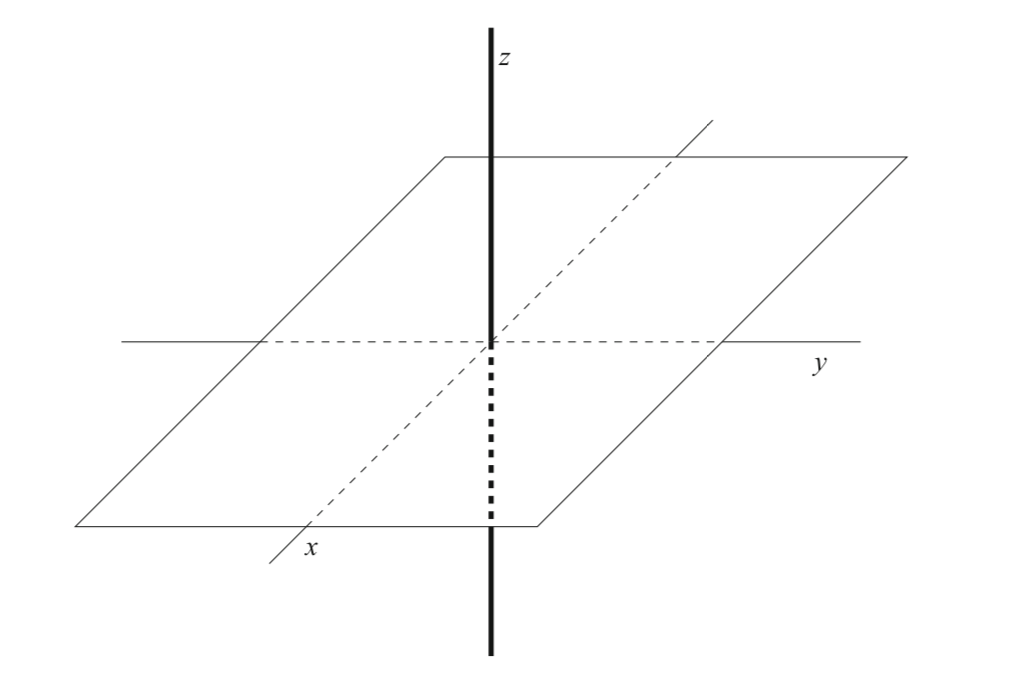
\includegraphics[width=1.0\textwidth]{affineVariety.png}
 	\caption[Example of an affine variety]{Affine variety defined by $(xz,yz)$. Image source: (\cite{algGeom}, page $9$).}
 	\label{fig1}
 \end{figure}

 \begin{DF}
Let $R$ be an commutative ring, then any non-empty subset $I \subseteq R$ is called a (two-sided) \textbf{ideal} of $R$ if it satisfies following requirements:
\begin{itemize}
\item $I \neq \emptyset,$\hfill ($I$ is a non-empty set)
\item $\forall f,g \in I: (f + g) \in I,$ \hfill ($I$ is closed under addition)
\item $\forall f \in I,\ \forall h \in R: hf \in I.$ \hfill ($I$ is closed under multiplication by $R$)
\end{itemize}
\end{DF}
\noindent In this thesis we are mostly concerned about ideals generated by a finite number of polynomials over some field.
\begin{DF}
Let $X = (x_1, \ldots ,x_n)$ be an ordered $n$-tuple of formal variables and let $f_1,\ldots,f_s \in \mathbb{F}[X] $ be an $s$-tuple of polynomials. Then we set
$$
\langle f_1, \ldots, f_x \rangle := \{ \sum_{i=1}^n h_if_i\ |\ h_1,\ldots,h_s \in \mathbb{F}[X]\}
$$
\end{DF}
\noindent to be the \textbf{ideal generated by} polynomials $f_1,\ldots,f_s$.
\begin{RM}
Every ideal $I$ of $\mathbb{F}[X]$ is finitely generated which means:
$$
\exists s \in \mathbb{N},\ \exists f_1,\ldots,f_s \in \mathbb{F}[X]: I = \langle f_1, \ldots, f_s \rangle,
$$
\noindent and we say that these polynomials $f_1,\ldots,f_s$ form a \textbf{basis} of $I$. Note that a given ideal $I$ may have many different bases. If we have two different bases $B_1 = (f_1,\ldots,f_s),\ s \in \mathbb{N},$ and $B_2 = (g_1, \ldots, g_t),\ t \in \mathbb{N},$ of the same ideal $I$ in $\mathbb{F}[X]$ such that $I = \langle B_1\rangle = \langle B_2 \rangle,$ then the affine varieties in $\mathbb{F}^n$ defined by the bases $B_1$ and $B_2$ are the same.
$$
\mathcal{V}(B_1) = \mathcal{V}(B_2).
$$
\end{RM}
\begin{DF}
Let $\mathcal{V} \subseteq \mathbb{F}^n$ be an affine variety and let $X = (x_1, \ldots ,x_n)$ be an ordered $n$-tuple of formal variables. Then we set 
$$
\mathbf{I}(\mathcal{V}) := \{ f \in \mathbb{F}[X]\ |\ \forall a \in \mathcal{V}: f(a) = 0\}.
$$
\noindent to be the \textbf{ideal of affine variety} $\mathcal{V}$.
\end{DF}
\begin{RM}
The natural question to ask is whether $\mathbf{I}(\mathcal{V}(f_1,\ldots,f_s)) = \langle f_1,\ldots,f_s \rangle.$ The answer, unfortunately, is not always yes, but the following set inclusion holds:
$$
\langle f_1,\ldots,f_s \rangle \subseteq \mathbf{I}(\mathcal{V}(f_1,\ldots,f_s)) .
$$
\end{RM} 
\begin{DF}
Let $f,g \in \mathbb{F}[x]$ be two non-constant polynomials of degrees $l,m \in \mathbb{Z}_{>0}$, deg$(f) = l,\ $deg$(g)=m$. Then $f,g$ have a common factor $\in \mathbb{F}[x]$ if and only if there are polynomials $A,B \in \mathbb{F}[x]$ such that:
\begin{enumerate}
\item $A \neq 0,\ B \neq 0,$ 
\item deg$(A) \leq m - 1,$ deg$(B) \leq l - 1,$
\item $Af  + Bg = 0.$
\end{enumerate}
\noindent To decide whether polynomials $f,g$ have a common factor, we can rewrite $Af  + Bg = 0$ as a system of linear equations and find a non-zero solution.
\begin{align*}
A &= u_0x^{m-1} + \cdots + u_{m-1}, \\
B &= v_0x^{l-1} + \cdots + v_{l-1}, \\
f &= c_0x^l + \cdots + c_l, \quad c_0 \neq 0, \\
g &= d_0x^m + \cdots + d_m, \quad d_0 \neq 0. \\
\end{align*}
If we compare the coefficients of powers of $x$, then we get a system of linear equations with variables $u_i,\ i \in \{0,1,\ldots	, m - 1\}$ and $v_j,\ j \in \{0,1,\ldots, l - 1\}$ and coefficients $c_i, d_j \in \mathbb{T}.$ The coefficient matrix of this system is called the \textbf{Sylvester matrix} of $f$ and $g$ with respect to $x$, denoted by Syl$_{x}(f,g)$. Syl$_{x}(f,g)$ is the following $(l + m) \times (l + m)$ matrix:
$$
\text{Syl}_{x}(f,g) := \begin{pmatrix}
c_0 &  &  &  &             d_0 &  &  &  \\
c_1 & c_0 &  &  &        d_1 & d_0 &   &  \\
c_2 & c_1 & \ddots &  & d_2 & d_1 & \ddots  &  \\
\vdots & & \ddots & c_0 & \vdots &  & \ddots & d_0 \\
 &  \vdots &  & c_1 &  & \vdots &  & d_1 \\
c_l &  &  &  &  d_m&  &  & \\
 & c_l &  & \vdots &  & d_m &  & \vdots \\
 &  & \ddots &  &  &  & \ddots &  \\
\coolunder{m \text{ columns}}{\hphantom{..} & \hphantom{...} & \hphantom{..}  & c_l & }\coolunder{l \text{ columns}}{\hphantom{...} & \hphantom{...} & \hphantom{......} & d_m \hphantom{..}} \\
\end{pmatrix}
$$
where the empty spaces are filled by zeros. \\
\noindent The determinant (we expect our reader is familiar with this term, if not, you can find its definition in any decent linear algebra textbook) of the Sylvester matrix is called the \textbf{resultant} of polynomials $f$ and $g$ with respect to $x$ and is denoted by Res$_{x}(f,g)$. Furthermore, $f,g$ have a common factor in $\mathbb{F}[x]$ if and only if Res$_x(f,g) = 0$. Example of the resultant of two quadratic polynomials is shown on page \pageref{resExample}. \\ \\
\noindent If $f,g$ have a common factor $h \in \mathbb{F}[x],\ \text{deg}(h) \geq 1$, then there exist $f_1, g_1 \in \mathbb{F}[x]$ such that:
$$
f = hf_1, \quad g = hg_1.
$$
\end{DF}
\noindent If $\mathbb{F}$ is an algebraically closed field, polynomials $f,g$ have a common root $r \in \mathbb{F}$. Since $\mathbb{F}$ is algebraically closed field, (non-constant) common factor $h$ has a root $r \in \mathbb{F}$: $h(r) = 0$ which implies $r$ is a common root of polynomials $f,g$:
\begin{align*}
(hf_1)(r) &= h(r)f_1(r) = 0f_1(r) = 0 \Leftrightarrow f(r) = 0 ,\\
(hg_1)(r) &= h(r)g_1(r) = 0g_1(r) = 0 \Leftrightarrow g(r) = 0.\\
\end{align*}

\subsection{Monomial Ordering}
\noindent The notion of ordering of terms in polynomial is a key ingredient in many algorithms, e.g. long division of polynomials. When dealing with polynomials in only one variable we usually write the terms of the polynomial in the decreasing order by their monomial degree. For example, $f(x) = 2x^4 - 10x^3 + x^2 + x -12$. The degree ordering on the one-variable monomials is straightforward:
$$
\cdots > x^{m+1} > x^m > x^{m-1} \cdots > x^2 > x > 1
$$
We would like to establish an ordering on the terms in polynomials in $\mathbb{F}[X],$ where $X = (x_1, \ldots, x_n)$. First, we note that we can reconstruct the monomial $X^{\alpha} = x_1^{\alpha_1}\cdots x_n^{\alpha_n}$ from the $n$-tuple of exponents $\alpha = (\alpha_1,\ldots, \alpha_n) \in \mathbb{Z}_{\geq 0}^n.$ Based on this observation we can define an ordering $>$ on the space $\mathbb{Z}_{\geq 0}^n$ which will also gives us an ordering on the monomials $\in \mathbb{F}[X].$ If for some $\alpha, \beta \in  \mathbb{Z}_{\geq 0}^n$ and some ordering $>$ holds: $\alpha > \beta$ we will also say that $X^\alpha > X^\beta.$ We will only consider \textbf{total orderings} which means that for every pair of monomials $X^\alpha$ and $X^\beta$, exactly one of the three statements holds:
\begin{itemize}
\item $X^\alpha > X^\beta,$\hfill (when $\alpha > \beta$)
\item $X^\alpha = X^\beta,$\hfill (when $\alpha = \beta$)
\item $X^\alpha < X^\beta,$\hfill (when $\alpha < \beta$)
\end{itemize}
\noindent and $>$ is transitive:
$$
\forall \alpha, \beta, \gamma \in \mathbb{Z}_{\geq 0}^n: (X^\alpha > X^\beta \land X^\beta > X^\gamma) \implies X^\alpha > X^\gamma.
$$
\noindent We also require that multiplication of two polynomials does not change the relative order of terms. Therefore the following property for $>$ must hold:
$$
\forall \alpha, \beta, \gamma \in \mathbb{Z}_{\geq 0}^n: X^\alpha > X^\beta \implies X^\alpha X^\gamma > X^\beta X^\gamma.
$$
\noindent Which in terms of the exponent vectors means: 
$$
\forall \alpha, \beta, \gamma \in \mathbb{Z}_{\geq 0}^n: \alpha > \beta \implies \alpha + \gamma > \beta + \gamma.
$$
\noindent To summarize all the requirements, we make the following definition.
\begin{DF}
A \textbf{monomial ordering} $>$ on $\mathbb{F}[X]$, where $X = (x_1, \ldots, x_n)$ is a relation $>$ on $\mathbb{Z}_{\geq 0}^n$ satisfying:
\begin{itemize}
\item $>$ is a total ordering on $\mathbb{Z}_{\geq 0}^n$,
\item $\forall \alpha, \beta, \gamma \in \mathbb{Z}_{\geq 0}^n: \alpha > \beta \implies \alpha + \gamma > \beta + \gamma,$
\item $\forall A \subseteq \mathbb{Z}_{\geq 0}^n,\ A \neq \emptyset: \exists \alpha \in A,\ \forall \beta \in A \setminus \{\alpha \}: \beta > \alpha.$ 
\end{itemize}
\noindent Last requirement tells us that in every non-empty subset of $\mathbb{Z}_{\geq 0}^n$ there exists a smallest element under the relation $>$.
\end{DF}
\phantom{.}
\phantom{.}
\noindent Now we will define a couple of standard monomial orderings.
\begin{DF}
Let $\alpha = (\alpha_1, \ldots, \alpha_n),\ \beta = (\beta_1, \ldots, \beta_n)\in \mathbb{Z}_{\geq 0}^n.$ \textbf{Lexicographic Order} (\textbf{lex}), denoted by $>_{lex}$, is a generalization of the way words are ordered in a dictionary. We say $\alpha >_{lex} \beta$ if the leftmost non-zero entry of the vector difference $\alpha - \beta \in \mathbb{Z}^n$ is positive. We will write: $X^\alpha >_{lex} X^\beta$ if $\alpha >_{lex} \beta$.
\end{DF}
For example:
\begin{itemize}
\item $(10,4,3) >_{lex} (10, 3, 4),$ since $\alpha - \beta = (0,1,-1)$.
\item $(7,5,3,1) >_{lex} (7, 5, 2, 4),$ since $\alpha - \beta = (0,0,1,-3)$.
\item The variables $x_1,\ldots,x_n$ are ordered in the usual way by the lexicographic order:
$$
(1,0,\ldots,0) >_{lex} (0,1,0,\ldots, 0) >_{lex} \cdots >_{lex} (0, \ldots, 0, 1),
$$
so $x_1 >_{lex} x_2 >_{lex} \cdots >_{lex} x_n.$ \\ \\
In the rest of the thesis we will also assume $x >_{lex} y >_{lex} z,$ unless stated otherwise.
\end{itemize} 
\begin{DF}
Let $\alpha = (\alpha_1, \ldots, \alpha_n),\ \beta = (\beta_1, \ldots, \beta_n)\in \mathbb{Z}_{\geq 0}^n.$ \textbf{Graded Lexicographic Order} (\textbf{grlex}), denoted by $>_{grlex}$, at first orders terms by the total degree, then break ties using the standard lexicographic order defined above. 
$$
\alpha >_{grlex} \beta: (|\alpha| > |\beta|) \lor (|\alpha| = |\beta| \land \alpha >_{lex} \beta),
$$
where $|\alpha| = \sum_{i=1}^n \alpha_i$ and $|\beta| = \sum_{i=1}^n \beta_i$.
\end{DF}
\begin{itemize}
\item $(10,2,6) >_{grlex} (10, 3,4),$ since $|\alpha| = 18 > |\beta| = 17$.
\item $(7,5,3,1) >_{grlex} (7, 5, 1, 3),$ since $|\alpha| = 16 = |\beta|$ and $\alpha >_{lex} \beta$.
\item The variables $x_1,\ldots,x_n$ are ordered the same way as by $>_{lex}$ order:
$$
(1,0,\ldots,0) >_{grlex} (0,1,0,\ldots, 0) >_{grlex} \cdots >_{grlex} (0, \ldots, 0, 1),
$$
\end{itemize} 
\begin{DF}
Let $\alpha = (\alpha_1, \ldots, \alpha_n),\ \beta = (\beta_1, \ldots, \beta_n)\in \mathbb{Z}_{\geq 0}^n.$ \textbf{Graded Reverse Lexicographic Order} (\textbf{grevlex}), denoted by $>_{grevlex}$, is somehow less intuitive order, but it is usually the most efficient for computations.  We say $\alpha >_{grevlex} \beta$ if $|\alpha| > |\beta|$ or if $|\alpha| = |\beta|$ and the rightmost non-zero entry of vector difference $\alpha - \beta \in \mathbb{Z}^n$ is negative.
\end{DF}
\begin{itemize}
\item $(4,7,1) >_{grevlex} (4, 2,5),$ since $|\alpha| = 12 > |\beta| = 11$.
\item $  (7, 5, 1, 3) >_{grevlex} (1,5,3,7),$ since $|\alpha| = 16 = |\beta|$ \\
\phantom{.}\hfill and $\alpha - \beta = (6,0,-2, -4),\ -4 < 0$.
\item The variables $x_1,\ldots,x_n$ are ordered the same way as by $>_{lex}$ order:
$$
(1,0,\ldots,0) >_{grevlex} (0,1,0,\ldots, 0) >_{grevlex} \cdots >_{grevlex} (0, \ldots, 0, 1),
$$
\end{itemize}
Now we will show how would the polynomial $f(x,y,z) = 4xy^2z + 4z^2 - 5x^3 + 7x^2z^2 \in \mathbb{Z}[x,y,z]$ be written if we reorder its terms by those standard monomial orderings.
\begin{itemize}
\item With respect to the lex order, we would reorder the terms of $f$ in decreasing order:
$$
f(x,y,z) = -5x^3 + 7x^2z^2 + 4xy^2z + 4z^2.
$$
\item With respect to grlex order:
$$
f(x,y,z) = 7x^2z^2  + 4xy^2z -5x^3 + 4z^2.
$$
\item With respect to grevlex order:
$$
f(x,y,z) = 4xy^2z + 7x^2z^2  -5x^3 + 4z^2.
$$
The first two terms have the same total degree of $4$ and $xy^2z >_{grevlex} x^2z^2$ because $(1,2,1) - (2,0,2) = (-1,2,-1)$ and $-1 < 0$.
\end{itemize} 
\begin{DF}
Let $f = \sum_\alpha a_\alpha X^\alpha$ be a non-zero polynomial in $\mathbb{F}[X]$ and let $>$ be a monomial order.
\begin{itemize}
\item The \textbf{multidegree} of $f$ is:
$$
\text{multideg}(f) := \text{max}(\alpha \in \mathbb{Z}_{\geq 0}^n\ |\ a_\alpha \neq 0),
$$
the maximum is taken with respect to $>$.\\ \\
Let $g \in \mathbb{F}[X],\ g \neq 0$, then multideg$(fg) = \text{multideg}(f) + \text{multideg}(g)$. If $(f + g) \neq 0$, then $\text{multideg}(f + g) \leq \text{max}(\text{multideg}(f),\ \text{multideg}(g))$, more precisely if the multidegrees of $f$ and $g$ are not equal, then the equality occurs: $\text{multideg}(f + g) = \text{max}(\text{multideg}(f),\ \text{multideg}(g))$.
\item The \textbf{leading coefficient} of $f$ is:
$$
\text{LC}(f) := a_{\text{multideg}(f)} \in \mathbb{F}.
$$
\item The \textbf{leading monomial} of $f$ is:
$$
\text{LM}(f) := X^{\text{multideg}(f)} \in \mathbb{F}[X],
$$
with coefficient $1$.
\item The \textbf{leading term} of $f$ is:
$$
\text{LT}(f) := (\text{LC}(f)\cdot \text{LM}(f)) \in \mathbb{F}[X].
$$
\end{itemize}
\end{DF}
\noindent To illustrate that, let $f(x,y,z) = 4xy^2z + 4z^2 - 5x^3 + 7x^2z^2 \in \mathbb{Z}[x,y,z]$ as before and lets use $>_{grevlex}$ order.
\begin{align*}
f(x,y,z) &= 4xy^2z + 7x^2z^2  -5x^3 + 4z^2, \text{ (in  grevlex order)}\\
\text{multideg}(f)&=(1,2,1), \\
\text{LC}(f)&=4, \\
\text{LM}(f)&=xy^2z, \\
\text{LT}(f)&=4xy^2z. \\
\end{align*}
Now we can formulate the idea of a general division algorithm in $\mathbb{F}[X]$.
\begin{RM}
Let $p, q \in \mathbb{F}[X]$ be two monomials, we say that the monomial $p$ is \textbf{divisible} by the monomial $q$ if and only if there exists a monomial $h \in \mathbb{F}[X]$ such that: $p = qh$. We denote it by $q\ |\ p$ which can be read  as \textbf{$\mathbf{q}$ divides $\mathbf{p}$}.
\end{RM}
\begin{DF}
Let $>$ be a monomial order on $\mathbb{Z}_{\geq 0}^n$, let $F = (f_1, \ldots, f_s)$ be an ordered $s$-tuple of polynomials in $\mathbb{F}[X],$ where $X = (x_1, \ldots, x_n)$. Then every $f \in \mathbb{F}[X]$ can be written as:
$$
f = q_1f_1 + \cdots + q_sf_s + r,
$$
where $q_i, r \in \mathbb{F}[X]$, and either $r = 0$ (is a zero polynomial) or $r$ is a linear combination, with coefficients in $\mathbb{F}$, of monomials $\in \mathbb{F}[X]$, none of those monomials is divisible by any of LT$(f_1), \ldots,$LT($f_s$).
We call polynomial $r$ a \textbf{remainder} of $f$ on division by $F$. Furthermore, if $q_if_i \neq 0$, then
$$
\text{multideg}(f) \geq \text{multideg}(q_if_i).
$$
\end{DF}
\noindent The algorithm itself will be presented in the chapter \ref{Algorithms}. Unfortunately,  the remainder is not uniquely characterized and depends on the order of the divisors in the set $F$ and also on the monomial order itself. \\ \\
\noindent Furthermore, we would like to use this idea to answer the ideal membership problem. Let $f, f_1, \ldots, f_s \in \mathbb{F}[X]$ and let $I = \langle f_1, \ldots, f_s \rangle$ be an ideal. We would like to determine whether $f \in I$ is true. We can clearly state that if the remainder $r$ obtained after division of $f$ by $F = (f_1, \ldots, f_s)$ is $0$, then $f$ has to be an element of the ideal $I$. So $r=0$ is a sufficient condition for the ideal membership, however it isn't a necessary condition for $f$ being in the ideal. To remedy this situation we will try to describe a "good" basis of the ideal $I$, such that the remainder $r$ on division by the polynomials of this basis will be uniquely determined and that the condition $r=0$ will be equivalent to the membership in the ideal. Exactly those good properties have Gröbner bases which we are gonna describe in the following section.
\section{Gröbner Bases}
\begin{DF}
An ideal $I \subseteq \mathbb{F}[X]$ is called a \textbf{monomial ideal} if there exists a (possibly infinite) subset $A \subseteq \mathbb{Z}_{\geq 0}^n$ such that $I$ consists of all polynomials which are finite sums: $\sum_{\alpha \in A} h_\alpha X^\alpha$, where $h_\alpha \in \mathbb{F}[X].$ We can then write $I$ in the form: $I = \langle X^\alpha \ |\ \alpha \in A\rangle.$ Monomial $X^\beta, \beta \in \mathbb{Z}_{\geq 0}^n,$ lies in ideal $I$ if and only if there exist $\alpha \in A$, such that $X^\alpha \ |\ X^\beta$ ($X^\beta$ is divisible by some $X^\alpha$). 
\end{DF}
\begin{RM}
\textbf{(Dickson's Lemma).} Any monomial ideal $I = \langle X^\alpha \ |\ \alpha \in A\rangle \subseteq \mathbb{F}[X]$ can be written in the form $I = \langle X^{\alpha(1)}, \ldots, X^{\alpha(s)}\rangle,\ s \in \mathbb{N},$ where $\alpha(1), \ldots, \alpha(s) \in A$. In particular, $I$ has a finite basis $(X^{\alpha(1)}, \ldots, X^{\alpha(s)})$.
\end{RM}
\begin{DF}
A monomial ideal $I \subseteq \mathbb{F}[X]$ has a finite basis $(X^{\alpha(1)}, \ldots, X^{\alpha(s)})$ with the property that $X^{\alpha(i)}$ does not divide $X^{\alpha(j)}$ for any $i \neq j$. Furthermore, this basis is unique and is called the \textbf{minimal basis} of $I$.
\end{DF}
\begin{DF}
Let $I \subseteq \mathbb{F}[X],\ I \neq {0},$ be an ideal and fix a monomial ordering on $\mathbb{F}[X]$.  Then:
\begin{itemize}
\item We denote by LT$(I)$ the \textbf{set of leading terms} of non-zero elements of~$I$.
$$
\text{LT}(I) = \{ cX^\alpha \ |\ \exists f \in I \setminus \{0\}: \text{LT}(f)= cX^\alpha \}.
$$
\item We denote by $\langle \text{LT}(I) \rangle$ the \textbf{ideal of leading terms} of $I$. $\langle \text{LT}(I) \rangle$ is a monomial ideal, therefore there exist a finite set $g_1,\ldots, g_t \in I,\ t \in \mathbb{N},$ such that:
$$
\langle \text{LT}(I) \rangle = \langle \text{LT}(g_1), \ldots, \text{LT}(g_t) \rangle.
$$
\end{itemize}
\end{DF}
\begin{DF}
Fix a monomial order on $\mathbb{F}[X]$, therefore every polynomial $f \in \mathbb{F}[X]$ has an unique leading term. A finite subset $G = \{g_1, \ldots, g_t \}$ of an ideal $I \subseteq \mathbb{F}[X],\ I \neq \{ 0 \}$ is said to be a \textbf{Gröbner basis} (or \textbf{standard basis}) if:
$$
\langle \text{LT}(g_1), \ldots, \text{LT}(g_t) \rangle = \langle \text{LT}(I) \rangle.
$$
Additionally we define the Gröbner basis of the zero ideal $\{0\}$ to be the empty set $\emptyset$ using the convention that $\langle \emptyset \rangle = \{0\}.$
\end{DF}
\begin{RM}
Every ideal $I \subseteq \mathbb{F}[X]$ has a Gröbner basis. Furthermore, any Gröbner basis for an ideal $I$ is a basis of $I$. The theory of Gröbner bases was developed by B. Buchberger in his PhD thesis (1965) and named after his thesis's advisor W. Gröbner. Buchberger also developed fundamental algorithms to find and work with Gröbner bases. In many computer algebra systems there is usually used an alternative spelling "Groebner bases".
\end{RM}
\phantom{.}
\phantom{.}
\noindent Now we will mention few important properties of Gröbner bases.
\begin{RM}
Let $I \subseteq \mathbb{F}[X]$ be an ideal and let $G = \{g_1, \ldots, g_t\}$ be a Gröbner basis of $I$. Then for any $f \mathbb{F}[X],$ there is an unique polynomial $r$ with those two properties:
\begin{itemize}
\item No term of $r$ is divisible by any of LT$(g_1),\ldots,$LT$(g_t)$.
\item $\exists g \in I:\ f = g + r.$
In particular, $r$ is the remainder on division of $f$ by set $G$ no matter how are the elements of $G$ listed when using the division algorithm. 
\end{itemize}
Polynomial $r$ is called the \textbf{normal form} of f. \\ \\ 
\noindent Polynomial $f \in I$ if and only if the remainder $r$ on division $f$ by $G$ is zero, $r = 0.$
\end{RM}
\begin{DF}
Let $f \in \mathbb{T}[X]$ be an polynomial and let $F = (f_1, \ldots, f_s) \subseteq \mathbb{T}[X]$ be an ordered $s$-tuple of polynomials. We will denote the remainder on the division of $f$ by $F$ by $\overline{f}^F$. If $F$ is a Gröbner basis for $\langle f_1, \ldots, f_s \rangle$, then we can regard $F$ as a set without any particular order, because the remainder on the division by a Gröbner basis is unique.
\end{DF}

%properties of GBases
%BCHberg criterium
%
%Define VectorSpace?
%Divison Res => alg in the next section with F4, F5
%
%Schoof–Elkies–Atkin algorithm - pocet bodu na EC 
\chapter{Elliptic Curves and Discrete Logarithm Problem}
\section{Elliptic Curves}
This section's main focus will be elliptic curves and groups of points on those elliptic curves. At first we are going to define what is a general elliptic curve, after that we will define an operation on the set of points on elliptic curve that with "the point in infinity" form an Abelian group. This section is based mostly on \cite{mky}.
\begin{DF}
An \textbf{elliptic curve} over a (prime order) finite field $GF(p),$ \\ $p > 3,\ p$ prime, defined by the short Weierstrass equation, is a set:
$$
E(GF(p)) := \{(x,y)\ |\ x,y \in \mathbb{T},\ y^2 = x^3 + Ax+B\} \cup \{ \mathcal{O} \},
$$
where $A, B \in GF(p)$ are \textbf{coefficients of the elliptic curve} and the \textbf{discriminant} of the elliptic curve, denoted by $\Delta$, is non-zero. Point $\mathcal{O}$ is called the \textbf{point at infinity} (in the projective plane).
\begin{align*}
\Delta = -16(4A^3 + 27B^2) \neq 0.
\end{align*}
Curves satisfying this condition are called \textbf{non-singular} and the right-hand-side polynomial ($x^3 + Ax+B$) in $x$ has 3 distinct roots. 
\end{DF}
\begin{DF}
Let $E(GF(p))$ be an elliptic curve and let $P,Q \in E(GF(p)),\ P=(x_1,y_1),\ Q=(x_2,y_2)$ be two points on the elliptic curve $E$. We define the binary operation $\oplus: E(GF(p)) \times E(GF(p)) \to E(GF(p))$, called \textbf{addition on the elliptic curve} $E(GF(p))$, as follows:
\begin{itemize}
\item Point at infinity $\mathcal{O}$ is an identity element of the operation $\oplus$, therefore if $P = \mathcal{O},\ P \oplus Q = Q,$ or if $Q = \mathcal{O},\ P \oplus Q = P.$
\item Else if $x_1 = x_2$ and $P\neq Q$, $P\oplus Q = \mathcal{O}.$ Point at infinity $\mathcal{O}$ is the identity element of the operation $\oplus$, therefore point $Q$ is the \textbf{additive inverse} of the point $P$, denoted by $\ominus P$. We can now state the explicit formula for the point $\ominus P$, we know its $x$-coordinate is $x_1$, and we will use the $E$ equation and substitute $X$ with $x_1$:
$$
Y^2  = (x_1^3 + Ax_1 + B),
$$
which is a quadratic equation in the variable $Y$ and we already know one of its roots, which is $y_1$, the other root has to be $-y_1$, therefore point $\ominus P = (x_1, -y_1).$
\item Else if $x_1 \neq x_2$, let $\lambda$ be the slope of the line defined by the points $P,Q.$
$$
\lambda = \frac{y_2 - y_1}{x_2 - x_1},
$$
else if $P = Q$ (\textbf{point doubling}), let $\lambda$ be the slope of the tangent line to the elliptic curve equation at the point $P.$
$$
\lambda = \mathlarger{\mathlarger{\frac{\frac{\mathrm{d}E}{\mathrm{d}X}}{\frac{\mathrm{d}E}{\mathrm{d}Y}}}}(x_1, y_1) = \frac{3x_1^2+ A}{2y_1}, 
$$
where $\frac{\mathrm{d}E}{\mathrm{d}X}, \frac{\mathrm{d}E}{\mathrm{d}Y}$ is the derivative of the elliptic curve equation with respect to $X,Y$. \\
The result of the operation $\oplus$ is:
\begin{align*}
x_3 &= \lambda^2 - x_1 - x_2, \\
y_3 &= \lambda(x_1 - x_3) - y_1, \\ 
 P \oplus Q &= (x_3, y_3).
\end{align*}
\end{itemize}
\end{DF}
\begin{DF}
A set of points on the elliptic curve defined by the short Weierstrass equation and the binary operation $\oplus$ form an Abelian group, $(E(GF(p)), \oplus)$ is a group and we denote it by $E$, or if we want to explicitly mention the coefficients $A,B$ and the prime field $GF(p),$ we use $E(A,B,p)$.
\end{DF}
\begin{NRM}
Let $P \in E$ be a point on an elliptic curve $E$ with group operation $\oplus$. To shorten the notation of the repeated application of the group law we will use the notation introduced in chapter 1. To remind our readers: \textbf{multiplication} of a point on the elliptic curve $E$ by an integer has the following meaning:
$$
\forall P \in E,\ \forall t \in \mathbb{Z}: tP := \begin{cases} \underbrace{P \oplus P \oplus \cdots \oplus P}_{\text{$t$-times}} &\quad t > 0, \\
\mathcal{O} \text{ (identity element) } &\quad t = 0, \\
\underbrace{(\ominus P) \oplus (\ominus P) \oplus \cdots \oplus (\ominus P)}_{\text{$t$-times}} &\quad t < 0.
\end{cases}
$$
\end{NRM} 
\begin{RM}
The complexity of arithmetic operations on $E$ is based on the complexity of operations in the underlying finite field $GF(p)$.  Exact number of arithmetic operations depends on the used algorithm and on the architecture of the CPU where it's executed. Table \ref{tblComp} provides a brief summary of the relationship between the operations on elliptic curve $E$ and number of arithmetic operations in the underlying finite field $GF(p)$. Addition in $GF(p)$ is denoted by $a_p$, multiplication in $GF(p)$ is denoted by $\cdot_p$, last column is the number of multiplicative inverses in $GF(p)^{\times}$. 
\begin{table}[!h]
\centering
\begin{tabular}{ |c||c|c|c| } 
 \hline
 & \# $+_p$ & \# $\cdot_p$ & \# mult. inverses \\ 
 \hline
 \hline
$\ominus P$ & 1 & 0 & 0  \\  \hline
$P \oplus Q, P \neq Q$ & 6 & 3 & 1 \\  \hline
$P \oplus Q, P = Q$ & 5 & 5 & 1 \\  \hline
$tP,\ t \in \mathbb{Z}_{\geq 0},\ k = \mathlarger{\lceil} \log_2(t) \mathlarger{\rceil}$ & $ (5k + 0.5k)$\footnotemark & $5k$ & 0 \\ \hline
\end{tabular}
\caption{Complexity of the arithmetic operations on the elliptic curve $E$ over $GF(p)$.}
\label{tblComp}
\end{table}
\end{RM}
\noindent We denote the number of bits of $p$ by $n = \mathlarger{\lceil} \log_2(p) \mathlarger{\rceil}$, then addition in $GF(p)^{+}$ is asymptotically $O(n)$, multiplication in $GF(p)^{\times}$, using Montgomery method \cite{handbook}, is $O(n^2)$ and multiplicative inverse in $GF(p)^{\times}$, using a careful implementation of the extended Euclidean algorithm (EEA) \cite{handbook}, is $O(n^2)$. An alternative to the EEA for calculating a multiplicative inverse in $GF(p)^{\times}$ is based on the Lagrange's theorem \ref{lagrange}. 
\begin{align*}
\forall a \in GF(p)^{\times},\ \exists n \in \mathbb{N}: \#a \cdot n = \#GF(p)^{\times} &= p - 1, \\ 
\forall a \in GF(p)^{\times}: a^{\#a} = 1 \implies a^{\#a - 1} &= a^{-1}, \\
\forall a \in GF(p)^{\times}: a^{-1} &= a^{p-2}.
\end{align*}
To calculate $a^{p-2}$ we can use the standard algorithm called square-and-multiply, for details see \cite{mky}, which has the same complexity $O(n^2)$ as the EEA.
\footnotetext{Using signed binary expansion of $t$ for the double-and-add algorithm, see \cite{mky} page 105.}
\begin{DF}

\end{DF}
\section{Discrete Logarithm Problem}
Let $y = b^x$, given $y \in \mathbb{R}_{> 0}$ and the base $b \in \mathbb{R}_{>0}$, we are asked to find the exponent $x \in \mathbb{R}$. We can rewrite this problem from the exponential form to the logarithmic form: $x = \log_b(y)$, to find the $x$ we can easily evaluate it on a calculator (using change of logarithm basis rule). Even if we didn't know the inverse function (logarithm), the exponential function is a strictly increasing function, therefore we could have just guessed a random $x_0$, evaluate $b^{x_0}$, compare it with $y$ and we would immediately know whether the solution $x$ is bigger/equal/lesser than $x_0$.
\\
\\
\noindent If we were given the same problem in a finite group, instead of over the real numbers, the situation would be significantly more complicated.
\begin{DF}
Let $G = (M, \cdot)$ be a group and let $h = g^x$, given $h \in M$ and the base $g \in M,\ \langle g \rangle = G,$ we are asked to find the exponent $x$~$\in$~$\{1, 2, \ldots, \#G\}.$ We call $x$ the \textbf{discrete logarithm} of $h$ with respect to the base $g$ and denote it by $x= \log_g(h)$. Problem of finding the solution $x$ is therefore called the \textbf{discrete logarithm problem} (DLP). We have decided to demand $g$ to be a generator of $G$ in order to guarantee the existence of the solution to the DLP.  
\end{DF}
\noindent To illustrate the difficulty of solving the DLP. Lets consider the multiplicative group $G$ of the finite field $GF(19).$ $G = (\{1,2,\ldots,18\}, \cdot_{19})$ and its generator $g=3,\ g \in G$. Group structure is shown on the figure \ref{fig2}. We might be asked to find such $k$, that $3^k \equiv 4 \text{ (mod 19)}$. 
 \begin{figure}[h]
\hspace*{-2cm}
 	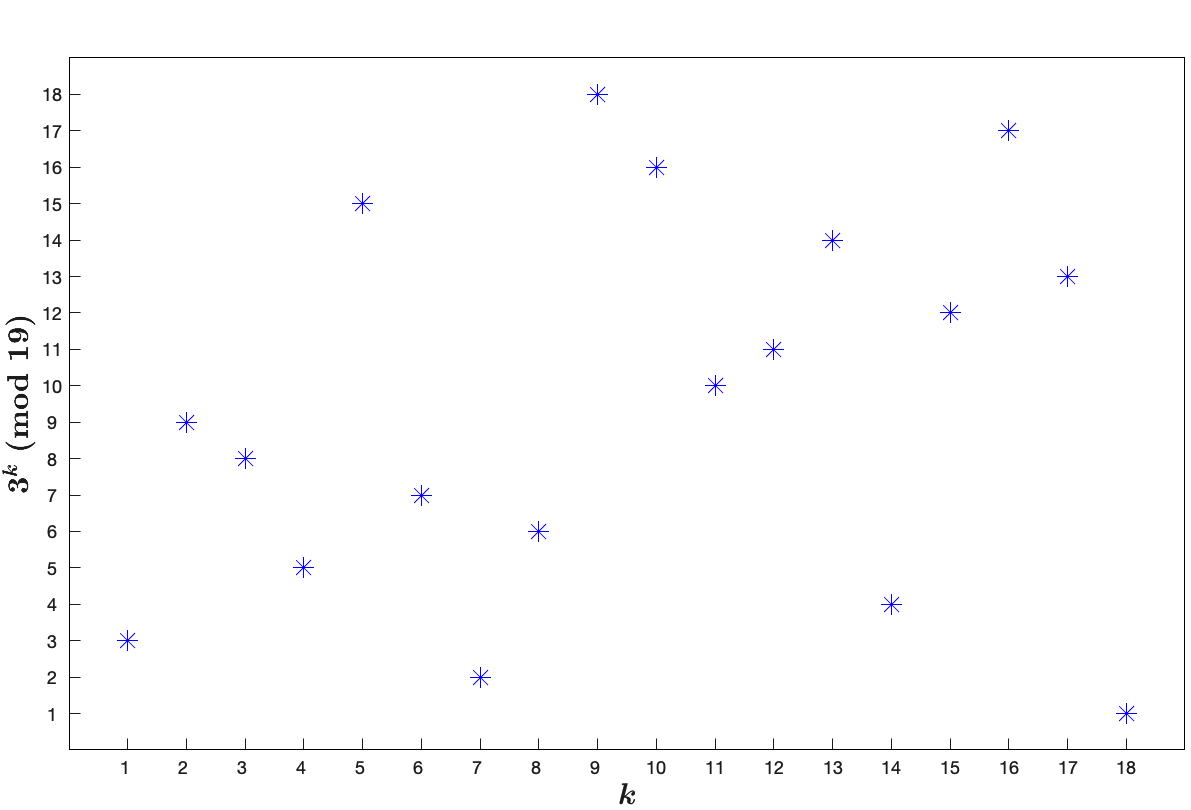
\includegraphics[width=1.25\textwidth]{graph3in19.png}
 	\caption[Example of the group structure of $GF(19)^\times$.]{Powers of the generator $g = 3$ in $GF(19)^\times$. Image was created by the author himself.}
 	\label{fig2}
 \end{figure}
 \newpage
\noindent Unfortunately, the function $g^k \text{ (mod 19)},\ k \in \mathbb{N},$ isn't monotonic, therefore we can't use the idea of trying a randomly selected $k_0$ and comparing $3^{k_0} \text{ (mod 19)}$ with $4$, but we can use the fact that the group $G$ is finite and its order is $\#G = 18 \implies 3^{18} \equiv 1 \text{ (mod 19)}.$ We can just try all possible values of $k \in \{0, 1, \ldots, 17\}$ and find the answer. This method is called the \textbf{brute-force attack}. 
\begin{align*}
3^0 \equiv 1 \text{ (mod 19)} &\not\equiv 4 \text{ (mod 19)}, \\
3^1 \equiv 3 \text{ (mod 19)} &\not\equiv 4 \text{ (mod 19)}, \\
3^2 \equiv 9 \text{ (mod 19)} &\not\equiv 4 \text{ (mod 19)}, \\
3^3 \equiv 8 \text{ (mod 19)} &\not\equiv 4 \text{ (mod 19)}, \\
&\vdots \quad \vdots \\
3^{13} \equiv 14 \text{ (mod 19)} &\not\equiv 4 \text{ (mod 19)}, \\
3^{14} &\equiv 4 \text{ (mod 19)}.
\end{align*}
The solution of this DLP is therefore $k = 14$ and we can see that the brute-force approach is very lengthy even for DLP in groups of small order. Complexity of solving the DLP in a group $G$ using the brute-force attack is $O(\#G)$ of group operations.
\begin{RM}
Standard properties of the logarithm may be used in the discrete logarithm case as well. Let $G$ be a finite Abelian group and let $g$ be a generator of $G$.
\begin{itemize}
\item $\forall p, q \in G: \log_g(pq) \equiv log_g(p) + log_g(q) \text{ (mod $\#G$)}$,
\item $\forall p, q \in G: \log_g(p(q)^{-1}) \equiv log_g(p) - log_g(q) \text{ (mod $\#G$)}$,
\item $\forall k \in \mathbb{Z},\ p \in G: \log_g(p^k) \equiv k \cdot log_g(p) \text{ (mod $\#G$)}$,
\item $h \in G,\ \langle h \rangle = G,\ \forall p \in G: log_g(p) \equiv log_h(p) \cdot log_g(h)  \text{ (mod $\#G$)}$.
\end{itemize}
Last property is the well-known change-of-base formula and tells us that if we are able to effectively solve the DLP with respect to some base we can use it to effectively solve the DLP with respect to any other base.
\end{RM}

\noindent Discrete logarithm problem can be stated in any group, the difficulty of solving it greatly depends on the group structure and the group operation. To solve the DLP we can develop a generic algorithm that works in any group and doesn't explore the group structure, or we can develop a specific algorithm for a chosen type of a group. For example, in an additive group $(\{0,1,\ldots, p-1\}, +_p)$, $p$ prime, we can solve the DLP in $O(\log^2(p))$ time using the extended Euclidean algorithm. Shoup proved that a generic algorithm to solve the DLP in a generic group of prime order $p$ would have to do $O(\sqrt{p})$ group operations \cite{shoup}. The best general algorithm to match this lower bound is Pollard's $\rho$ (rho) algorithm, described in the subsection \ref{polard}. 
\\
\\
\noindent The main focus of this thesis is to solve the DLP stated on an elliptic curve using a specific algorithm. 
\begin{DF}
Let $E$ be an elliptic curve over a prime field $GF(p)$, let $P$ be a generator of $E$ and let $Q$ be a second point on $E$. \textbf{Elliptic curve discrete logarithm problem} (ECDLP) is to find an integer $k \in \{1,2,\ldots	, \#E\}$ such that $Q = kP$.
\end{DF}
\section{Generic algorithms for solving ECDLP}
In this section we will describe three most known generic algorithms for solving the DLP, we will use the elliptic curve notation. The first algorithm is based on collision finding, time complexity is lower than for a naive brute-force algorithm, but we the memory requirements are significant. This section was based mostly on \cite{mky}.
\subsection{Baby-step Giant-step Algorithm (BsGs)}
\begin{DF}
\textbf{(Baby-step Giant-step)}: Let $E$ be an elliptic curve group over $GF(p)$, equipped with operation $\oplus$, $P \in E$ its generator and $xP = Q \in G,\ x \in \{0, 1, \ldots, \#E - 1\}$, we will denote the order of $E$ by $N = \#E$. We know, based on Hasse's theorem (\ref{hase}), for large $p$, $N$ is approximately $p$. Following algorithm solves the ECDLP in $O(\sqrt{N})$ group operations $\oplus$.
\begin{itemize}
\item Let $n = \mathlarger{\mathlarger{\mathlarger{\lceil}}} \sqrt{N} \mathlarger{\mathlarger{\mathlarger{\rceil}}}$, we will pre-compute a list of length $n$ of multiples of $P$.
\item $0P = \mathcal{O}, P, 2P, \ldots, (n-1)P,$ \hfill (baby-step phase) \\
next generate multiples of $Q$ and try to find it in the list generated in the baby-step phase.
\item $Q \oplus (0\cdot n \ominus P) = Q, Q \oplus (1\cdot n \ominus P), Q \oplus (2\cdot n \ominus P), \ldots, Q \oplus ((n-1)\cdot n \ominus P),$\\
This is called the giant-step phase.
\item If there is a collision for some $iP$ and $Q \oplus (j\cdot n \ominus P)$, we can solve the ECDLP and find $x$:
\begin{align*}
iP = Q \oplus (j\cdot n \ominus P) \implies i &\equiv x + (-jn) \text{ (mod $N$)} \\
x &\equiv i + jn \text{ (mod $N$)}.
\end{align*}
\end{itemize}
\noindent The algorithm is deterministic and is guaranteed to find the solution, because it basically tries all the possible values of $x$. Every number in $\{0, 1, \ldots, N - 1\}$ can be expressed as $i + jn,\ n = \mathlarger{\mathlarger{\mathlarger{\lceil}}} \sqrt{N} \mathlarger{\mathlarger{\mathlarger{\rceil}}},i,j \in \{0,1,\ldots, n-1\}.$ 
For the efficient implementation it's crucial to be able to effectively find a collision in the pre-computed list, therefore it's advisable to use a hash table, to achieve the constant time lookup. If that is satisfied the algorithm time complexity is $O(\sqrt{N})$ of group operations and space complexity is $O(\sqrt{N})$.
\end{DF}
\noindent For example, let $E = E(1,1,29)$ be an elliptic curve group over $GF(29)$ and its elliptic curve equation is $y^2 = x^3 + x + 1$. Let $P = (24,25)$ be a generator of $E$, let $Q \in E$, we want to find an integer $x$ such that: $Q = xP.$ Order of $E$ is 36, so we will set $n = 6$ and pre-calculate the baby-step list:
\begin{center}
\begin{tabular}{ |c||c|c|c|c|c|c| }
\hline
$i$ & 0 & 1 & 2 & 3 & 4 & 5\\ \hline
 $iP$ & $\mathcal{O}$ & $(24,25)$ &  $(6,7)$ & $(0,28)$ & $(10,24)$ & $\textbf{(28,12)}$ \\ \hline
\end{tabular}
\end{center}
This step depends only on the group $E$ and its generator $P$, we can pre-calculate it only once and reuse it for different points $Q$. Let solve the ECDLP in this group for $Q = (18,15)$. We will now iterate over multiples of $Q$ and look for a collision in the pre-calculated list.
\begin{center}
\begin{tabular}{ |c||c|c|c|c|c|c| }
\hline
$j$ & 0 & 1 & 2 & 3 & 4 & 5\\ \hline
 $Q\oplus(6j\ominus P)$ & $(18,15)$ & $(11,3)$ &  $(12,1)$ & $(8,17)$ & $\mathbf{(28,12)}$ & $(24,4)$ \\ \hline
\end{tabular}
\end{center}
We have found a collision for $j=4$ and $i=5$ (in the pre-computed list):
$$
5P = Q\oplus(24\ominus P) \implies 4 \equiv x -24 \text{ (mod 36)} \implies x \equiv 29  \text{ (mod 36)}.
$$
We can now verify that $29P = (18,15) = Q.$
\subsection{Pollard $\mathbf{\rho}$-Algorithm}
\noindent The main drawback of the BsGs algorithm is its space complexity, we need to store $\sqrt{\#E}$ elliptic curve points. To remedy this problem, in 1978 John Pollard published a different algorithm, which is called after him the Pollard~$\rho$(rho)-algorithm, with the same time complexity as BsGs but with very little memory requirements. A similar algorithm can be used for factoring composite integers. This subsection is based on \cite{mky}.
\begin{DF}
\label{pol}
 \textbf{(Pollard $\mathbf{\rho}$ algorithm)}: Let $S$ be a finite set of $N$ elements, let $f: S \to S$ be a function. Choose $x_0 \in S$ a starting point of the sequence defined by: $x_i = (\underbrace{f\circ f \circ \cdots \circ f}_\text{$i$-times})(x_0)$, then there exists $L \in \mathbb{N}$ such that:
 $$
 x_{2i} = x_i, \quad 1\leq i < L.
 $$
Set $S$ is finite, therefore for some $k \in \mathbb{N}_{< N}$ the sequence $x_0, x_1, \ldots, x_k$ has to a point that repeats twice in this sequence, we denote the first such point by $x_T$, it's clear that after that point the sequence is in a cycle of length $M$, where $T+M$ is the index of the second occurrence of the point $x_T$ in the sequence. To prove the existence of $i$ such that: $x_{2i} = x_i$ we can start with the fact that: $\forall k \in \{0, 1, \ldots, M-1\}: x_{T+k} = x_{T+k+M},$ which implies:
$$
\exists i \geq T,\ i < T + M: 2i \equiv i \text{ (mod $M$)} \implies i\ |\ M.
$$
The argument is simple, in every sequence of $M$ consecutive integers there has to be exactly one that is divisible by $M$, therefore we can see that the $L$ in the definition \ref{pol} is in fact $L= T + M \leq N$. On average (with different choices of $x_0$ and function $f$) it takes $O(\sqrt{N})$ steps to obtain a collision with a probability over 50\% (based on the birthday paradox), for a thorough analysis see \cite{polProb}. \\ \\
\noindent For a graphical illustration see figure \ref{rho}, the first point in the sequence that repeats itself twice is $x_3$, therefore we set $T = 3$, and the length of the cycle is $M = 6$, because $x_T = x_3 = x_{3+6}$. The only integer in the set $\{3,4,5,6,7,8\}$ that is divisible by $M = 6$ is $6$, therefore $i=6$ and we can easily verify that $x_6 = x_{2*6} = x_{12}$. The graph \ref{rho} has a strong resemblance to the Greek letter $\rho$, hence the name of the algorithm.
 \begin{figure}[h]
 \centering
 \hspace*{-1cm}
 	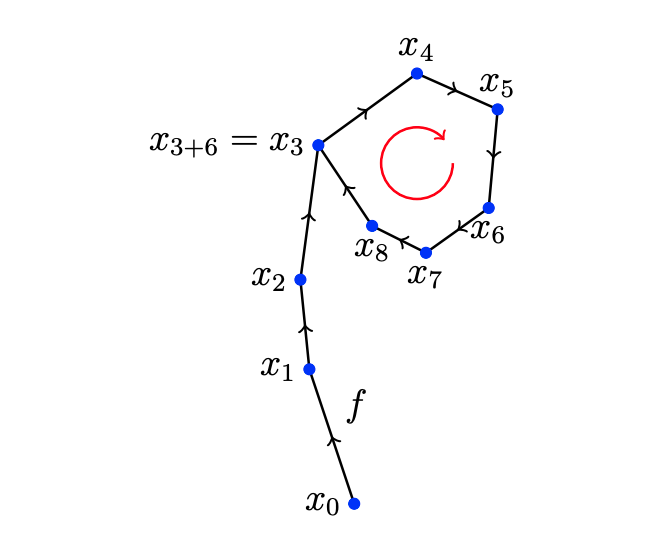
\includegraphics[width=1\textwidth]{rho.png}
 	\caption[Graphical illustration of Pollard $\rho$ collision idea.]{Graphical illustration of the idea behind the Pollard $\rho$ algorithm. $T = 3$, length of the cycle $M = 6$. Image source: (\cite{mky}, page $70$).}
 	\label{rho}
 \end{figure}
 \end{DF}
 \begin{DF}
 The Pollard $\rho$ algorithm might be used to solve the ECDLP. Let $E$ be an elliptic curve group with points' coordinates $\in GF(p)$, let $P$ be its generator and let $Q \in E$ be some other point. We want to find $x=\log_P(Q)$. Let denote the order of $E$ by $N := \#E$. We divide $E$ into three disjunctive sets $S_1, S_2, S_3$, so that $\mathcal{O} \not\in S_2$ and for $i \in \mathbb{Z}_{\geq 0}$ define $f: E \to E$:
 $$
 T_{i+1} = f(T_i) := \begin{cases} P \oplus T_i,\quad T_i \in S_1, \\
 2T_i, \quad T_i \in S_2, \\
 Q \oplus T_i, \quad T_i \in S_3.
 \end{cases}
 $$
 We can start with $T_0 = \mathcal{O}$, so after $k$ steps we get:
 $$
 T_k = (\underbrace{f\circ f \circ \cdots \circ f}_\text{$k$-times}(\mathcal{O}) = \alpha_k P \oplus \beta_k Q.
 $$
 We need to keep track of $\alpha_k,\ \beta_k$, so we set $\alpha_0 = \beta_0 = 0$ and define it recursively for $k \in \mathbb{Z}_{\geq 0}$:
$$ 
  \alpha_{k+1} := \begin{cases} \alpha_k + 1\text{ (mod $N$)},\quad T_k \in S_1, \\
 2\alpha_k\text{ (mod $N$)}, \quad T_k \in S_2, \\
 \alpha_k, \quad T_k \in S_3.
 \end{cases}
$$
$$ 
  \beta_{k+1} := \begin{cases} \beta_k,\quad T_k \in S_1, \\
 2\beta_k\text{ (mod $N$)}, \quad T_k \in S_2, \\
 \beta_k + 1\text{ (mod $N$)}, \quad T_k \in S_3.
 \end{cases}
$$
We also create a second sequence of points on elliptic curve $E$: $R_0 = \mathcal{O},\forall k \in \mathbb{N}: R_k := T_{2k} = \gamma_kP \oplus \delta_kQ$, we also need to keep track of $\gamma_k,\ \delta_k$. After some number of steps ($i$) we will encounter a collision: $R_i = T_{2i} = T_i$, then we have a relation: 
$$
\gamma_iP \oplus \delta_iQ = \alpha_iP \oplus \beta_iQ.
$$
Let $d = \text{gcd}(\beta_i - \delta_i, N)$, if $d=1$ we can easily find the solution $x$ to the ECDLP:
$$
x \equiv (\gamma_i - \alpha_i)\cdot(\beta_i - \delta_i)^{-1} \text{ (mod $N$)}.
$$
If $d \neq 1$ and is small it might be worthy to to find a solution $y$ mod($\frac{N}{d}$) in the same fashion:
$$
y \equiv (\gamma_i - \alpha_i)\cdot(\beta_i - \delta_i)^{-1} \text{ $\bigg($mod $\frac{N}{d}\bigg)$}, 
$$then we can find $x$ in the set:
$$
\bigg\{y + k\cdot\frac{N}{d}\ \bigg| \ k \in \{0, 1, \ldots, d -1\}\bigg\}.
$$
For $N$ prime $d$ will be small, if $N$ is not small and $d$ is not small we can restart the algorithm with a different partitioning $S_1,S_2,S_3$ or a different starting point $T_0$. Another option is to use the Pohlig-Hellman algorithm and solve multiple ECDLPs in prime subgroups and then find the final solution $x$ using the Chinese remainder theorem (CRT).
\end{DF}
\noindent For example, let $E = E(11,18,29)$ be an elliptic curve group over $GF(29)$ and its elliptic curve equation is $y^2 = x^3 + 11x + 11$. Let $P = (1,1)$ be a generator of $E$, let $Q \in E$, we want to find an integer $x$ such that: $Q = xP.$
Order of $E$ is 29 (prime). We divide elliptic curve points into sets $S_1,S_2,S_3$ based on their $x$-coordinates:
$$
\forall R = (R_x, R_y) \in E: \begin{cases} R \in S_1, \quad \text{ if } 0\leq R_x < \big\lfloor\frac{p}{3}\big\rfloor, \\ 
R \in S_2, \quad \text{ if } \big\lfloor\frac{p}{3}\big\rfloor \leq R_x < 2\big\lfloor\frac{p}{3}\big\rfloor, \\
R \in S_3, \quad \text{ if } 2\big\lfloor\frac{p}{3}\big\rfloor \leq R_x, 
\end{cases}
$$ where $p = 29.$ 
Set $S_1$ contains the identity element $\mathcal{O}$. Cardinalities of the sets are following $|S_1| = 9,\ |S_2| = 12, \ |S_3| = 8.$ \\
Lets solve the ECDLP for $Q=(13,26)$. In the table \ref{tblRho} are shown the intermediate results of the algorithm.
\begin{table}[!h]
\centering
\begin{tabular}{ |c||c|c|c|c|c|c| } 
\hline
$i$ & $\alpha_i$ & $\beta_i$ & $T_i$ & $\gamma_i$ & $\delta_i$ & $R_i$ \\ 
\hline
\hline
0 & 0 & 0 & $\mathcal{O}$ &  0 & 0 & $\mathcal{O}$ \\ \hline
1 & 1 & 0 & $(1,1)$ &  2 & 0 & $(18,25)$ \\ \hline
2 & 2 & 0 & $(18,25)$ &  3 & 1 & $(3,22$ \\ \hline
3 & 2 & 1 & $(5,13)$ &  8 & 2 & $(11,7)$ \\ \hline
4 & 3 & 1 & $(3,22)$ &  3 & 8 & $(8,3)$ \\ \hline
5 & 4 & 1 & $(12,14)$ &  4 & 9 & $(13,3)$ \\ \hline
6 & 8 & 2 & $(11,7)$ &  8 & 19 & $(13,3)$ \\ \hline
7 & 16 & 4 & $(14,4)$ &  16 & 10 & $(13,3)$ \\ \hline
8 & 3 & 8 & $(8,3)$ &  3 & 21 & $(13,3)$ \\ \hline
9 & 4 & 8 & $(26,25)$ &  6 & 14 & $(13,3)$ \\ \hline
10 & 4 & 9 & $\mathbf{(13,3)}$ &  12 & 0 & $\mathbf{(13,3)}$ \\ \hline
\end{tabular}
\caption{Intermediate values of the Pollard $\rho$ algorithm.}
\label{tblRho}
\end{table}
\\
\noindent After 10 iterations we have found a collision: 
$$
4P + 9Q = 12P \implies x \equiv 8\cdot9^{-1} \text{ (mod $29$)} \equiv 17 \text{ (mod $29$)}. 
$$
We can now verify that $17P = (13,26) = Q.$
\subsection{Pohlig-Hellman Algorithm}
As we have mentioned in the previous subsection, Pollard $rho$ algorithm works the best in a prime order group. In a case when order of a group $G$ is a composite number $N$ with small factors, we can solve multiple ECDLPs in subgroups of prime order and then using the CRT find the final solution. This algorithm was presented in 1978 by Stephen Pohlig and Martin Hellman in their article \cite{PH}. 
\begin{DF} (\textbf{Chinese Remainder Theorem} (CRT)): Let $m_i \in \mathbb{N},\ i \in \{1,\ldots, k\},$ be mutually relatively prime integers, and $N=\prod_{i=1}^k m_i,\ x_i \in \mathbb{Z},\ i \in \{1,\ldots, k\}.$ 
The following system of congruences:
\begin{align*}
x &\equiv x_1 \text{ (mod $m_1$)}, \\
x &\equiv x_2 \text{ (mod $m_2$)}, \\
&\vdots \quad \vdots \\
x &\equiv x_k \text{ (mod $m_k$)},
\end{align*}
has a solution $c$:
$$
c = \sum_{i=1}^k x_iN_iM_i,
$$ where $N_i=\frac{N}{m_i}$ and $M_i\equiv(N_i)^{-1} \text{ (mod $m_i$)}$ and any other solution $c'$ is congruent to $c$ modulo $N$.
\end{DF}
\begin{DF}(\textbf{Pohlig-Hellmann algorithm}): Let $E$ be an elliptic curve group of composite order $N$ and let the factorization of $N$ be:
$$
N = \prod_{i=1}^kp_i^{e_i},\ \forall i \in \{1, 2, \ldots, k\}: e_i \in \mathbb{Z}_{\geq 0},\ p_i \text{ is prime}.
 $$ Let $P$ be a generator of $E$ and let $Q \in E$, we want to find an integer $x$ such that: $xP = Q$. We can split this ECDLP into multiple ECDLPs in a prime power subgroups. 
 \begin{itemize}
 \item For each $i \in \{1, 2, \ldots, k\}$ let:
 $$
 P_i := \frac{N}{p_i^{e_i}}P, \quad Q_i := \frac{N}{p_i^{e_i}}Q.
 $$ Each $P_i$ is a generator of an elliptic curve subgroup of prime power order  $\#P_i = p_i^{e_i}.$ In this subgroup we will solve the ECDLP, find an integer $x_i$  such that: $x_iP_i = Q_i.$
 \item  For each $i \in \{1, 2, \ldots, k\}$ we will solve the ECDLP in a prime power subgroup.  We may rewrite the unknown integer $x_i := y_{i,0} + y_{i,1}p_i + y_{i,2}p_i^2+ \cdots + y_{i,e-1}p_i^{e_i-1}.$ We can now repeatedly solve the ECDLP in a prime subgroup to obtain one unknown digit of $x_i$ by shifting the rest of them out. To find the first digit $y_{i,0}$ we will multiply both sides of the equation by $p_i^{e_i-1}$:
\begin{align*}
p_i^{e_i-1} Q_i &= p_i^{e_i-1}\cdot x_i  P_i\\ 
&= p_i^{e_i-1}\cdot (y_{i,0} + y_{i,1}p_i + y_{i,2}p_i^2+ \cdots + y_{i,e-1}p_i^{e_i-1})P_i \\
&= p_i^{e_i-1}y_{i,0}P_i \oplus p_i^{e_i}\cdot\underbrace{(y_{i,1} + y_{i,2}p_i+ \cdots + y_{i,e-1}p_i^{e_i-2})P_i}_{\in \langle P_i \rangle} \\
&= y_{i,0}p_i^{e_i-1}P_i, \quad \text{(because }\forall T \in \langle P_i \rangle : p_i^{e_i}T = \mathcal{O})
\end{align*}
We may now solve the ECDLP in a prime subgroup of order $p_i$ generated by $p_i^{e_i-1}P_i$ and obtain first digit $y_{i,0}.$ Now we can move to the next digit $y_{i,1}$:
\begin{align*}
p_i^{e_i-2} Q_i &= p_i^{e_i-2}\cdot x_i  P_i\\ 
&= p_i^{e_i-2}\cdot (y_{i,0} + y_{i,1}p_i + y_{i,2}p_i^2+ \cdots + y_{i,e-1}p_i^{e_i-1})P_i \\
&= (p_i^{e_i-2}y_{i,0} + p_i^{e_i-1}y_{i,1})P_i \oplus p_i^{e_i}\cdot\underbrace{y_{i,2}+ \cdots + y_{i,e-1}p_i^{e_i-3})P_i}_{\in \langle P_i \rangle} \\
&= y_{i,0}p_i^{e_i-2}P_i \oplus y_{i,1}p_i^{e_i-1}P_i \implies \\
p_i^{e_i-2}(Q_i \ominus y_{i,0}P_i) &= y_{i,1}p_i^{e_i-1}P_i.
\end{align*}
To find the next digit $y_{i,1}$ we just need to solve the ECDLP in a prime subgroup of order $p_i$. We continue in the same fashion until all digits of $x_i$ are found.
\item Finally we solve the following system of congruences
\begin{align*}
x &\equiv x_1 \text{ (mod $p_1^{e_1}$)}, \\
x &\equiv x_2 \text{ (mod $p_2^{e_2}$)}, \\
&\vdots \quad \vdots \\
x &\equiv x_k \text{ (mod $p_k^{e_k}$)},
\end{align*}
using the CRT to obtain the final solution $x$.
\end{itemize}
\end{DF}
In the individual phase when we are solving the ECDLP in a prime order subgroup we can use any algorithm, usually BsGs or Pollard $\rho$ are used. The time complexity of Pohlig-Hellman algorithm is therefore (for more information see \cite{mky}):
$$
O\bigg(\sum_{i=1}^k\bigg[e_i\big(S(p_i) + \log(p_i)\big)\bigg]\bigg),
$$ where $S(p_i)$ is the time complexity of the algorithm used to solve the ECDLP in the prime subgroup of order $p_i$. For elliptic curve groups of order with small factors is Pohlig-Hellman significantly faster than the BsGs or Pollard $\rho$ (we often need to run it more than once with different starting points if the order is composite).
\noindent For example, let $E = E(1,2,75941)$ be an elliptic curve group over $GF(75941)$ and its elliptic curve equation is $y^2 = x^3 + x + 2$. Let $P = (64579,62139)$ be a generator of $E$, let $Q \in E$ be a point on elliptic curve $E$, we want to find an integer $x$ such that: $Q = xP.$ Order of $E$ is $76428 = 2^2\cdot 3^2\cdot 11 \cdot 193$. We will solve this problem using Pohling-Hellman algorithm. Let $Q = (1447, 50835)$.
\begin{table}[!h]
\centering
\begin{tabular}{ |c||c|c|c|c|c| } 
\hline
 $i$ & $p_i$ & $e_i$ & $P_i$ & $Q_i$ & $x_i$  \\
\hline
\hline
1 & 2 & 2 & $19107P = (1, 75939)$ &  $19107Q = (1,2)$ & 3  \\ \hline
2 & 3 & 2 & $8492P = (55693, 45178)$ &  $8492Q = (17273,40444)$ & 2 \\ \hline
3 & 11 & 1 & $6948P = (39499, 25804)$ &  $6948Q = (29264,5197)$ & 9 \\  \hline
4 & 193 & 1 & $396P = (58124, 73147)$ &  $396Q = (34502,8697)$ & 189 \\ \hline
\end{tabular}
\caption{Intermediate values of Pohlig-Hellman algorithm stating individual ECDLPs in prime power subgroups.}
\label{tblPH}
\end{table}
For $i=1,2$ we need to solve the ECDLP in a subgroup of prime square order. In the subgroup of order $2^2$ generated by $P_1 = (1, 75939)$, we can rewrite the unknown $x_1$ as $x_1 = y_{1,0} + 2y_{1,1}$, to find the first digit $y_{1,0}$ we will use the relation:
\begin{align*}
2Q_1 &= y_{1,0}\cdot2P_1 \\
(75940, 0) &= y_{1,0}(75940, 0) \implies y_{1,0} = 1.
\end{align*}
To find the second digit $y_{1,1}$ we will use the relation:
\begin{align*}
Q_1 \ominus y_{1,0}\cdot P_1 &= y_{1,1}\cdot 2P_1 \\
(1,2) \oplus (1,2) & = y_{1,1}(75940, 0) \\
(75940, 0) &= y_{1,1}(75940, 0) \implies y_{1,1} = 1.
\end{align*}
Therefore, $x_1 = y_{1,0} + y_{1,0}\cdot 2 = 1 + 2 = 3.$ In reality we could have just tried all four possible values for $x_1$. We will repeat the whole process in the subgroup generated by $P_2 = (55693, 45178)$ of order $3^2$. We rewrite the unknown integer $x_2$ as $x_2 = y_{2,0} + 3y_{2,1}$, to find the first digit $y_{2,0}$ we will use the relation:
\begin{align*}
3Q_2 &= y_{2,0}\cdot 3P_2 \\
(35655, 11621) &= y_{2,0}(35655, 64320) \implies y_{2,0} = 2.
\end{align*}
To find the second digit $y_{2,1}$ we will use the relation:
\begin{align*}
Q_2 \ominus y_{2,0}\cdot P_2 &= y_{2,1}\cdot 3P_2 \\
Q_2 \ominus 2P_2 &= y_{2,1}\cdot (35655, 64320) \\
\mathcal{O} &= y_{2,1}\cdot (35655, 64320) \implies y_{2,1} = 0.
\end{align*}
Therefore, $x_2 = 2 + 0\cdot 3 = 2$. In this case there are nine possible values for $x_2$, so in reality we could have easily tried them all. Now we can put the system of congruences together and solve it to find the final solution $x$.
\begin{align*}
x &\equiv 3 \text{ (mod $4$)}, \\
x &\equiv 2 \text{ (mod $9$)}, \\
x &\equiv 9 \text{ (mod $11$)}, \\
x &\equiv 189 \text{ (mod $193$)}, \\
\end{align*}
\begin{table}[!h]
\centering
\begin{tabular}{ |c||c|c|c|c| } 
\hline
 $i$ & $x_i$ & $m_i$ & $N_i$ & $M_i$ \\
\hline
\hline
1 & 3 & 4 & 19107 &  3 \\ \hline
2 & 2 & 9 & 8492 & 2\\ \hline \hline
3 & 9 & 11 & 6948 & 8 \\ \hline
4 & 189 &193 & 396 & 58 \\ \hline
\end{tabular}
\caption{Intermediate values of the CRT phase of the Pohlig-Hellman algorithm.}
\label{tblPH3}
\end{table}
\noindent Using the CRT we compute $x$ (the intermediate values are in the table \ref{tblPH3}):
$$
x \equiv 3\cdot 19107 \cdot 3 + 2\cdot 8492 \cdot 2 +  9\cdot 6948 \cdot 8 +  189\cdot 396 \cdot 58 \text{ (mod  76428)} \equiv 2891\text{ (mod  76428)}.
$$ We can now verify that $2891P = (1447, 50835) = Q.$
\section{Index Calculus for ECDLP}
The Index Calculus is originally a \textbf{subexponential} algorithm to solve the DLP in the multiplicative group of a finite field. 
\begin{DF}
Let $0\leq a \leq 1,\ a \in \mathbb{R}$ and $c \in \mathbb{R}_{>0}$. The \textbf{subexponential function} for the parameters $a$ and $c$ is:
$$
L_N(a,c) := \exp(c\log(N)^a \log(\log(N))^{1-a}).
$$
Let $N$ be a $k$-bit integer, note that taking $a=0$ gives $L_N(0,c) = \log(N)^c = k^c$ (polynomial) while taking $a=1$ gives $L_N(1,c) = N^c = \exp(ck)$ (exponential). Hence $L_N(a,c)$ interpolates exponential and polynomial growth. An algorithm is called \textbf{subexponential} when it's complexity is $O(L_N(a,c))$ with $0 < a < 1$, for more context see chapter 15 in \cite{subExp}.
\end{DF} 
\noindent However it is common to use the name index calculus algorithm to refer to any algorithm that operates in the same fashion as the original Index Calculus algorithm, which solves the DLP by collecting relations index calculus algorithm and using linear algebra afterwards \cite{amadori17}.
\begin{DF}
\textbf{Index Calculus for ECDLP}: Let $E$ be an elliptic curve over a prime order field $GF(p)$, let $P$ be a generator of $E$ and for simplicity we assume $\#P$ is prime (if it's not the case we can using the Pohlig-Hellman idea and split the ECDLP into multiple ECDLPs in prime subgroups). Let $Q \in E$, we want to find an integer $x$ such that $xP = Q$. The simplest version of index calculus algorithm consists of two main stages: the relation collection step and the linear algebra step. At first, we need to collect the relations:
\begin{enumerate}
\item Specify a factor base $\mathcal{F} \subset E$ such that we can effortlessly test the membership of an element to this factor base. 
\item Generate a random linear combination of points $P,Q$: 
$$
R := uP + vQ,\quad \text{$u,v$ are random integers from $GF(\#P)$}.
$$
\item If possible, express $R$ as a linear combination of the elements of the factor base $\mathcal{F}$:
\begin{align*}
R &= uP + vQ = \sum_{k=1}^{|\mathcal{F}|}a_k P_k,\quad \forall k \in \{1,2,\ldots,|\mathcal{F}|\}: P_k \in \mathcal{F},\ a_k \in GF(\#P), \\
\mathcal{O} &= -uP - vQ + \sum_{k=1}^{|\mathcal{F}|}a_k P_k.
\end{align*}
\item If $R$ cannot be expressed in terms of the factor base $\mathcal{F}$, continue with step 2. Otherwise, store the coordinates of $R$ with respect to $\mathcal{F}$ and integers $u,v$ as a row in the relation matrix $M$. The row is stored in this form:
$$
(a_1, a_2, \ldots, a_{|\mathcal{F}|}, -u, -v).
$$
\item We repeat this procedure (steps 2 to 4) until the end condition is met.
\end{enumerate}
\noindent Some authors (see \cite{amadori17} page 2) suggest end condition to set to number of decomposed points $R$ to be at least $|\mathcal{F}|$, but we need to state that this condition doesn't guarantee these relations are enough to solve the ECDLP. Another option, which guarantees we will be able to solve the ECDLP in the next step, is to collect relations until the rank of matrix $M$ is $|\mathcal{F}| + 1$, which is also the maximum rank this matrix can have (assuming $Q \neq \mathcal{O}$). We will state a weaker (that usually requires less relations to be found) end condition in the following section \ref{betterCond}. \\ \\
\noindent After collecting enough relations, the linear algebra step solves the ECDLP:
\begin{enumerate}
\item Matrix $M$ is over $GF(\#P)$, we will reduce it to row echelon form (using some linear algebra technique, e.g. Gaussian Elimination Method), the last non-zero row of the reduced matrix will look like $(0,0,\ldots, 0, 1, -v')$, which describes a relation:
\begin{align*}
\mathcal{O}  &= 1P \oplus (-v'Q) \\
P &= v'Q \implies x \equiv (v')^{-1} \text{ (mod $\#P$)}.
\end{align*}
We can always recover this solution $x$, because order of $\#P$ is prime and $P \neq \mathcal{O} \implies v' \not\equiv 0 \text{ (mod $\#P$)}$.
\end{enumerate}
\end{DF}
The main bottleneck of this algorithm lies in the decomposition of a point $R$ into the factor basis $\mathcal{F}$, usually known as \textbf{point decomposition problem} (PDP). Therefore, in order for this algorithm to be efficient, we require the solution of the PDP to be efficient (including the case when $R$ can't be decomposed into elements of $\mathcal{F}$) and we also require high success rate of the decomposition of $R$. Both there requirements are deeply affected by the choice of factor base $\mathcal{F}$ and its size \cite{amadori17}. \\ 

\subsection{Summation Polynomials}
\noindent In 2004 Igor Semaev published an article introducing summation polynomials in order transform the PDP to a problem of finding a solution of a multivariate polynomial equation based on the group law of a specific elliptic curve, for more information see the original article \cite{semaev04}.
\begin{DF}
Let $E$ be the elliptic curve given by the short Weierstrass equation over a prime field $\mathbb{F} = GF(p),\ p > 3$. For any natural number $n \geq 2$ let $S_n = S_n(X_1, X_2, \ldots, X_n)$ be a polynomial in $n$ variables which is related to the group operation on $E$. We call this polynomial the $n$-th \textbf{summation polynomial} and define it by the following property. Let $x_1,x_2,\ldots,x_n$ be any elements from $\overline{\mathbb{F}}$, the algebraic closure of the field $\mathbb{F}$, then $S_n(x_1,x_2,\ldots,x_n)=0$ if and only if there exist $y_1,y_2,\ldots,y_n \in \overline{\mathbb{F}}$ such that points $(x_i,y_i), \forall i \in \{1,2,\ldots,n\}$ are in the elliptic curve group defined by $E$ over $\overline{\mathbb{F}}$ and their sum is the identity element of this elliptic curve group:
$$
\mathcal{O} = \sum_{i=1}^n (x_i,y_i).
$$
For $n=2$ the summation polynomial is defined as: 
$$
S_2(X_1, X_2) := X_1 - X_2,
$$ it comes from the fact that 
$$
\forall P, Q \in E(A,B,p): P \oplus Q = \mathcal{O} \implies  Q = \ominus P.
$$
Based on the definition of the additive inverse in $E(A,B,p)$ we know, the points $P = (x_1,y_1)$ and $\ominus P = (x_1, -y_1)$ have the same $x$-coordinate which is equivalent to $S_2(x_1, x_2) = 0 \implies x_1 = x_2.$ To determine $S_3(X_1,X_2,X_3),$ let $(x_1,y_1)$ and $(x_2, y_2)$ be two affine ($\neq  \mathcal{O}$) points on $E(A,B,p$ such that $x_1 \neq x_2.$ We denote their sum and difference by:
\begin{align*}
(x_3,y_3) &:= (x_1,y_1) \oplus (x_2,y_2),\\
(x_4,y_4) &:= (x_1,y_1) \ominus (x_2,y_2).\\
\end{align*}
We will use the group law $\oplus$ to express $x_3$ and $x_4$ in terms of $x_1,x_2, y_1, y_2$:
\begin{align*}
x_3 &= \lambda_3^2 - (x_1 + x_2), \text{ where } \lambda_3 = \frac{y_2 - y_1}{x_2 - x_1},\\ 
x_4 &= \lambda_4^2 - (x_1 + x_2), \text{ where } \lambda_4 = \frac{y_2 + y_1}{x_2 - x_1}, \text{ since } \ominus (x_2,y_2) = (x_2, -y_2),\\ 
\end{align*}
To find a polynomial such that $x_3$ and $x_4$ are its roots, recall \textbf{Vieta's formulas}, let $z_1, z_2$ be two roots of the polynomial $p(z) = az^2 + bz + c$, then it has to satisfy following formulas:
$$
z_1 + z_2 = -\frac{b}{a},\quad z_1z_2 = \frac{c}{a}.
$$
Therefore, we want to find $x_3 + x_4$ and $x_3 x_4$:
\begin{align*}
x_3 + x_4 &= \lambda_3^2 + \lambda_4^2 - 2(x_1+x_2) \\
&= \frac{(y_2-y_1)^2 + (y_2+y_1)^2 -2(x_1+x_2)(x_2-x_1)^2}{(x_2-x_1)^2} \\
&= \frac{2y_2^2+2y_1^2 -2(x_1+x_2)(x_2-x_1)^2}{(x_2-x_1)^2}, \text{ (substite for $y_1^2,y_2^2$ using $E$ eq.)} \\
&= \frac{2(x_1^3+Ax_1+B+x_2^3+Ax_2+B) -2(x_1^3+x_2^3-x_1^2x_2-x_1x_2^2)}{(x_2-x_1)^2}\\
&= 2\frac{(Ax_1+Ax_2+2B) +x_1^2x_2+x_1x_2^2}{(x_2-x_1)^2} \\
&= 2\frac{x_1(x_1x_2 + A) + x_2(x_1x_2 + A)+2B}{(x_2-x_1)^2}\\ 
&= 2\frac{(x_1 + x_2)(x_1x_2 + A)+2B}{(x_2-x_1)^2}.
\end{align*}
\begin{align*}
x_3x_4 &= \frac{\bigg((y_2-y_1)^2 -(x_1^3+x_2^3-x_1^2x_2-x_1x_2^2)\bigg)\bigg((y_2+y_1)^2-(x_1^3+x_2^3-x_1^2x_2-x_1x_2^2)\bigg)}{(x_2-x_1)^4} \\
&= \frac{\bigg(y_1^2 + y_2^2 -2y_1y_2 -x_1^3-x_2^3+x_1^2x_2+x_1x_2^2\bigg)\bigg(y_1^2 + y_2^2 +2y_1y_2 -x_1^3-x_2^3+x_1^2x_2+x_1x_2^2\bigg)}{(x_2-x_1)^4}\\
&= \frac{\bigg(x_1^2x_2 + x_1x_2^2 + Ax_1 + Ax_2 - 2y_1y_2 + 2B\bigg)\bigg(x_1^2x_2 + x_1x_2^2 + Ax_1 + Ax_2 + 2y_1y_2 + 2B\bigg)}{(x_2-x_1)^4}\\
&= \frac{- 4 y_{1}^{2} y_{2}^{2} + x_{1}^{2} x_{2}^{4} + 2 x_{1}^{3} x_{2} A + 4 x_{1}^{2} x_{2}^{2} A + 2 x_{1} x_{2}^{3} A + x_{1}^{2} A^{2} + 2 x_{1} x_{2} A^{2} + x_{2}^{2} A^{2}}{(x_2-x_1)^4} \\
&+ \frac{4 x_{1}^{2} x_{2} B + 4 x_{1} x_{2}^{2} B + 4 x_{1} A B + 4 x_{2} A B + 4 B^{2} + x_{1}^{4} x_{2}^{2} + 2 x_{1}^{3} x_{2}^{3}}{(x_2-x_1)^4} \\
&= \frac{\bigg((x_1-x_2)^2\bigg)\bigg(x_{1}^{2} x_{2}^{2} - 2 x_{1} x_{2} A + A^{2} - 4 x_{1} B - 4 x_{2} B\bigg)}{(x_2-x_1)^4}, \text{ (substited for $y_1^2,y_2^2$ using $E$ eq.)}\\
&= \frac{(x_1x_2-A)^2 - 4B(x_1+x_2)}{(x_2-x_1)^2}.
\end{align*}
Therefore, the $x_3$ and $x_4$ are roots of the polynomial:
$$
f(X) := (x_2-x_1)^2X^2-2\bigg((x_1+x_2)(x_1x_2 + A) + 2B\bigg)X + \bigg((x_1x_2-A)^2 - 4B(x_1+x_2)\bigg).
$$
In the case $x_1=x_2$ one of points $(x_3,y_3), (x_4,y_4)$ is $2(x_1,y_1)$ and the other one has to be $\mathcal{O}$, without loss of generality, let's consider $(x_3,y_3) = 2(x_1,y_1)$ we will show that $x_3$ is the root of the polynomial $f(X)$.
\begin{align*}
x_1 = x_2:\ f(X) &= -2\bigg(2x_1(x_1^2+A)+2B\bigg)X +\bigg((x_1^2-A)^2-8Bx_1\bigg),
\\ X &= \frac{(x_1^2-A)^2-8Bx_1}{4(x_1^3+Ax_1+B)} \\ 
	X &= \frac{x_1^4-2Ax_1^2-8Bx_1+A^2}{4(x_1^3+Ax_1+B)}. \\
	x_3 &= \lambda^2 -2x_1, \quad \lambda = \frac{3x_1^2+A}{2y_1} \\
	x_3 &= \frac{9 x_{1}^{4} + 6 Ax_{1}^{2} + A^{2} -8x_1y_1^2}{4y_1^2}, \text{ (substitute for $y_1^2$ using $E$ eq.)} \\
	x_3 &= \frac{9 x_{1}^{4} + 6A x_{1}^{2} + A^{2}-8 x_{1}^{4} - 8 x_{1}^{2} A - 8B x_{1}}{4(x_1^3+Ax_1+B)} \\
	x_3 &= \frac{x_1^4-2Ax_1^2 - 8Bx_1+ A^2}{4(x_1^3+Ax_1+B)}. \\
\end{align*}
Therefore we can define the third summation polynomial as follows:
\begin{align*}
S_3(X_1,X_2,X_3) &:= (X_2-X_1)^2X_3^2-2\bigg((X_1+X_2)(X_1X_2 + A) + 2B\bigg)X_3\\
&+ (X_1X_2-A)^2 - 4B(X_1+X_2).
\end{align*}
$S_3$ is symmetric polynomial of degree $2$ in each variable $X_1,X_2,X_3$. $S_3$ is absolutely irreducible, for a proof and more information about summation polynoamials see \cite{semaev04}. In the same article Semaev also defined $n$-th summation polynomials (using resultant) for an arbitrary $n$ as follows:
\begin{align*}
\forall k,n \in \mathbb{N},\ n \geq 4,\ n-3\geq k \geq 1:\ S_n(X_1,X_2,\ldots, X_n) := \\ \text{Res}_y\bigg(S_{n-k}(X_1,\ldots,X_{n-k-1},y),\ S_{k+2}(X_{n-k},\ldots,X_n,y)\bigg).
\end{align*}
For example, 
\begin{align*}
S_4(X_1,X_2,X_3,X_4) &= \text{Res}_y\bigg(S_3(X_1,X_2,y),\ S_3(X_3,X_4,y)\bigg), \\
S_3(X_1,X_2,y) &= c_0y^2 + c_1y + c_2, \text{ where } \\
c_0 &= (X_2-X_1)^2,\\ 
c_1 &= -2\bigg((X_1+X_2)(X_1X_2 + A) + 2B\bigg),\\
c_2 &=  (X_1X_2-A)^2 - 4B(X_1+X_2),  \\
S_3(X_3,X_4,y) &= d_0y^2 + d_1y + d_2, \text{ where } \\
d_0 &= (X_4-X_3)^2,\\ 
d_1 &= -2\bigg((X_3+X_4)(X_3X_4 + A) + 2B\bigg),\\
d_2 &=  (X_3X_4-A)^2 - 4B(X_3+X_4), \\
S_4(X_1,X_2,X_3,X_4) &= \text{det}
\begin{pmatrix}
c_0 & 0 & d_0 & 0 \\
c_1 & c_0  & d_1 & d_0  \\
c_2 & c_1 &  d_2 & d_1 \\
 0 & c_2 & 0 & d_2 \\
\end{pmatrix}.
\end{align*}
\end{DF}
\label{resExample}
\noindent If we recall that resultant of two polynomials with respect to variable $y$ is zero if and only if both polynomials (over an algebraically closed field) have a common root. We can see that summation polynomials $S_{n-k}(X_1,\ldots,X_{n-k-1},y)$ and $S_{k+2}(X_{n-k},\ldots,X_n,y)$ are tied together with variable $y$, because if there exist $x_1,\ldots, x_n, y_0$ ($y_0$ is the common root of $S_{n-k}(y)$ and $S_{k+2}(y)$) such that:
\begin{align*}
S_{n-k}(x_1,\ldots,x_{n-k-1}, y_0) = 0 \land S_{k+2}(x_{n-k},\ldots,x_{n}, y_0) &= 0 \implies\\ \exists P_1,\ldots,P_n, (y_0, y_1) \in E(\overline{\mathbb{F}}): P_1 \oplus \cdots \oplus P_{n-k-1} \oplus (y_0,y_1) &= \mathcal{O}, \\
\exists v \in \{0,1\}: P_{n-k} \oplus \cdots \oplus P_{n} \oplus (-1)^{v}(y_0,y_1) &= \mathcal{O} \implies \\P_1 \oplus \cdots \oplus P_{n-k-1} \oplus (-1)^{v+1}\bigg(P_{n-k} \oplus \cdots \oplus P_{n}\bigg) &= \mathcal{O} \implies \\
S_n(x_1,\ldots,x_n) &= 0.
\end{align*}
\noindent Summation polynomials for $n \geq 3,\ n \in \mathbb{N}$ are symmetric, absolutely irreducible and of degree $2^{n-2}$ in each variable $X_i,\ i \in \{1,\ldots,n\}$.\\ \\
However, the higher summation polynomials are hardly practical (compared to $S_3$), because the growth of their degrees (in each variable) is exponential with respect to $n$. In 2015 Semaev himself presented a \textit{splitting trick}, a way how to transform $n$-th summation polynomial into a polynomial system of $S_3$ summation polynomials which can be solved more efficiently \cite{semaev15}. This trick is based on the resultant properties and the idea of tying multiple polynomial equations together with \textbf{bounding variables}. 
\begin{DF}\textbf{(The splitting trick)}: The roots of the $n$-th summation polynomial $S_n(X_1,\ldots,X_n)$ in $\overline{\mathbb{F}}[X_1,\ldots,X_n]$ are equivalent to the solutions of the following polynomial system:
\begin{align*}
&S_3(X_1,X_2,U_1) = 0, \\
&S_3(X_{k+2}, U_{k}, U_{k+1}) = 0, \quad 1 \leq k \leq n-4,\ k \in \mathbb{N}, \\
&S_3(X_{n-1}, X_n, U_{n-3}) = 0.
\end{align*} 
We call the variables $U_i,\ i \in \{1, \ldots, n - 3\}$ bounding variables. Therefore, by introducing $n-3$ new variables we obtain a polynomial system that consists of $n-2$ symmetric polynomials (each only in three variables) of degree two in each its variable instead of a single polynomial in $n$ variables of degree $2^{n-2}$ in each of its $n$ variables.
\end{DF}
\noindent Summation polynomials reduce the PDP to the solution of a system of multivariate polynomial equations which are usually solved by calculating the Gröbner basis of the ideal generated by those polynomial equations. This ideal $I$ is zero-dimensional, the set of common zeroes of the polynomials in $I$ is finite in $\overline{\mathbb{F}}$, which is equivalent to the fact that, for each variable $X_i,\ i \in \{1,\ldots,n\}$ there is a polynomial in the Gröbner basis for $i$, with a power of $X_i$ as a leading monomial \cite{FGLM}. Reduced Gröbner basis of the ideal spanned by those polynomial equations is either calculated with respect to the lexicographic order of monomials or is calculated with respect to some other order and then then converted using the FGLM algorithm to a Gröbner basis for the same ideal with respect to a different monomial order, for detailed information about this algorithm see \cite{FGLM}.
\begin{DF}
\label{triagForm}
Let $G = \{g_1,\ldots,g_s\}$ be the reduced basis for a zero-dimensional ideal $I \subset \mathbb{F}[X_1,\ldots,X_n]$ with respect to lex order with $X_1 >_{\text{lex}} \cdots >_{\text{lex}} X_n$ and ordered so that every LT$(g_j) >_{\text{lex}} $LT($g_{j+1}$). Then for each $i \in \{1,\ldots,n\}$ there is some $j=j(i)$ for which LT$(g_j)=x_i^{d_i}$ for some $d_i > 0.$ This is called the \textbf{triangular form} and is especially convenient for finding all the points that lie in the affine variety defined by the polynomials $g_1,\ldots,g_n$. \\ \\
\noindent The last polynomial in the Gröbner basis $G$ is univariate: $g_s = g_s(X_n)$, we find its roots and substitute them into other polynomials in $G$, after such substitution, at least one of the earlier polynomials $g_i,\ i \in \{1,\ldots,s-1\}$ is univariate in $X_{n-1}$. This is called \textbf{backsolving} or \textbf{backsubstitution}, for more information see~\cite{week11}.
\end{DF}
\noindent In the next chapter we describe specific algorithms solving ECDLP that were implemented and tested by us. The experimental results are in the chapter~\ref{expResults}.
\chapter{Specialized Algorithms Solving ECDLP}
In this chapter we first describe four specialized algorithms for solving ECDLP that are based on the theoretical concepts presented in the previous chapters. Afterwords, we follow up with the actual implementation's details. The experimental results are presented in chapter~\ref{expResults}.
\section{Algorithm 1 (Semaev 2015)}
Algorithm 1 is based on the Semaev's algorithm presented in \cite{semaev2015}, few changes had to be made to make the algorithm work for ECDLP over finite fields $GF(p),\ p$ prime. Semaev's algorithm works best over prime field extensions, where the base field is of prime characteristic $q,\ q \leq 2^{10}$ ( approximately).  \\ \\
\noindent Let $P$ be a generator of the prime order ($\#P = r$) group $E(GF(p))$, where $E$ is an elliptic curve defined over prime field $GF(p)$, $p$ prime. We are restricting this algorithm to the case where $E(GF(p))$ is a group of prime order, because if it's not the case, we can use the Pohlig-Hellman algorithm to split the initial ECDLP in the group of composite order to a multiple smaller ECDLPs in prime order subgroups, where algorithm 1 can be used to find the solution. The ECDLP is given a generator $P$ and some other point $Q \in E(GF(p))$, find an integer $k$ such that $kP = Q,$ since $E(GF(p))$ is a finite group of prime order $r$ we are interested in the solution $k\ \text{(mod }r)$. For large $p$, $r \approx p$. Algorithm 1, which computes this integer $k$, works in multiple steps and is described below.
\begin{enumerate}
\item Define the decomposition constant $m \geq 2,\ m \in \mathbb{N},$ and a factor base $\mathcal{F} \subset GF(p)$ of size $\mathlarger{\Big\lceil \sqrt[m]{r} \Big\rceil}$, where $\lceil \cdot \rceil$ is the ceiling function. The factor base $\mathcal{F}$ might consist of random $x$-coordinates of points on the elliptic curve $E$ (non-deterministic):
$$
\mathcal{F} := \Big\{x\ \Big|\ x \in GF(p),\ \exists y \in GF(p): (x,y) \in E(GF(p))  \Big\},
$$
or we can take the $|\mathcal{F}|$ smallest $x$-coordinates of points on the elliptic curve $E$ (deterministic).
\item Construct a relation matrix $M \in GF(r)^{|\mathcal{F}| + 1 \times |\mathcal{F}| + 2}$, $r$ is prime, therefore there exists a finite field of order $r$. Lets order elements of $\mathcal{F}$ and denote the $i$-th element of the factor base $\mathcal{F}$ by $\mathcal{F}_i,\ i \in \{0,\ldots,|\mathcal{F}| - 1\}.$
\begin{align*}
&\begin{matrix}
\hphantom{........}\mathbf{\mathcal{F}_0} & \hphantom{.......} \mathbf{\mathcal{F}_1} & \hphantom{...}\ldots &\hphantom{...} \mathbf{\mathcal{F}_{\mathcal{F} - 1}} & \hphantom{....}\mathbf{a} & \hphantom{......} \mathbf{b}
\end{matrix}\\
M := &\begin{pmatrix}
m_{1,1} & m_{1,2} & \ldots & m_{1,|\mathcal{F}|} & a_1 & b_1 \\
\vdots & \vdots & \cdots & \vdots & \vdots  & \vdots  \\
\hphantom{.}m_{|\mathcal{F}| + 1,1} & m_{|\mathcal{F}| + 1,2} & \ldots & m_{|\mathcal{F}| + 1,|\mathcal{F}|} & a_{|\mathcal{F}| + 1} & b_{|\mathcal{F}| + 1} \hphantom{.}
\end{pmatrix},
\end{align*}
where all elements of the matrix $M$ are in $GF(r)$. Each row of this matrix represents a relation in the group $E(GF(p))$:
$$
\forall j \in \{1,\ldots,|\mathcal{F}| + 1\}: a_jP \oplus b_jQ \oplus \sum_{i=1}^{\mathcal{F}} m_{j,i} (\mathcal{F}_{i-1}, y_{i-1}) = \mathcal{O}, 
$$
where $y_k,\ k \in \{0,\ldots,|\mathcal{F}| - 1\}$ is smaller of the $y$-coordinates of the points on $E$ with $x$-coordinate equal to $\mathcal{F}_k$ (if there is a point $(\mathcal{F}_k, y)$ in $E(GF(p))$ there is also its additive inverse $(\mathcal{F}_k,-y) = (\mathcal{F}_k, p - y)$ in $E(GF(p))$. We take smaller of these two values as $y_k := \text{min}(y, p - y)$.  \\ \\
The matrix $M$ is initialized as a zero matrix and we gradually fill it with relations. And initialize the row index $rowID = 1$ telling us where to insert the next found relation.
\item For random integers $a,b \in \{0, \ldots, r-1\}$ compute point ${R = aP \oplus bQ.}$ If $R = \mathcal{O}$ and $b \neq 0$ we can immediately solve the ECDLP:
$$k \equiv  (-a)(b)^{-1} \text{ (mod $r$)}.$$ Otherwise, $R$ has affine coordinates $(R_x, R_y)$. If $R_x = \mathcal{F}_k,$ for some $k \in \{0,\ldots,|\mathcal{F}| - 1\},$ then we have a relation and we add to the relation matrix $M$.
\begin{align*}
M_{rowID,\ k} &=\begin{cases} 1, \quad &R_y < \frac{p}{2}, \\
p-1, \quad &R_y > \frac{p}{2}.
\end{cases}\\
M_{rowID,\ |\mathcal{F}| + 1} &= a_{rowID} = b, \\
M_{rowID,\ |\mathcal{F}| + 2} &= b_{rowID} = a, \\
rowID &= rowID + 1.
\end{align*}
Otherwise, we try to decompose this point as a sum of factor base $\mathcal{F}$ points by solving following multivariate polynomial system, compute $x_1,\ldots,x_m \in \mathcal{F}$ and $u_1,\ldots,u_{m-2} \in GF(p)$ such that:
\begin{align*}
S_3(x_1,x_2,u_1) &= 0, \\
S_3(x_{k+2},u_k,u_{k+1}) &= 0,\quad 1 \leq k \leq m - 3,\ k \in \mathbb{N}, \\
S_3(x_m,R_x,u_{m-2}) &= 0, \\
\Bigg[\prod_{i=0}^{|\mathcal{F}| -1}\Big(x_j - \mathcal{F}_i\Big)\Bigg] &= 0, \quad  j \in \{1, \ldots, m\},
\end{align*}
the last $m$ products is used to restrict found solutions $x_1,\ldots,x_m$ to lie in the factor base $\mathcal{F}$. \\ 
\noindent Semaev also suggested adding the \textbf{field equations}:
$$
x_j^p - x_j = 0, \quad j \in \{1, \ldots, m\},
$$
which is not computationally feasible for large $p$ (approximately $p \geq 2^{10}$), so we won't generally use them (unless stated otherwise). Lets denote the set of the polynomials described above as $T$. Ideal $I = \langle T \rangle$ is a zero-dimensional ideal. Therefore, we can compute its Gröbner basis $G$ with respect to lexicographic order $X_1 >_{lex} >_{lex} \cdots >_{lex} X_n$ and by definition \ref{triagForm} it will be in a triangular form, so we can easily find the affine variety $\mathcal{V}(G) = \mathcal{V}(T)$, the set of the common zeroes of the polynomials in the set $T$. For every found solution ${(s_1, \ldots, s_m) \in GF(p)^m}$ we add update one row in the relation matrix:
$$
$$
\item 
\end{enumerate}

%$$\bigg[\prod_{\mathcal{F}_i \in V_j}\Big(x_j - \mathcal{F}_i\Big)\bigg] = 0, \quad  j \in \{1, \ldots, m\},\ i \in \{0, \ldots, |\mathcal{F}| - 1\},$$
%where $V_j$ are pair-wise disjoint sets of approximately the same size of factor base elements, $\forall j \in \{1, \ldots, m\}: |V_j| \approx \frac{|\mathcal{F}|}{m},\ V_j \subset \mathcal{F},$ it is used to restrict found solutions $x_1,\ldots,x_m$ to lie in the factor base $\mathcal{F}$. Each $x_i$ lies in the set $V_i$



%\begin{DF}
%\textbf{The splitting trick}: Let $E(GF(p))$ be an elliptic curve defined by the elliptic curve equation (in the short Weierstrass form) over a prime field $\mathbb{T} = GF(p)$. 
%The $n$-th summation polynomial $S_n$ is a polynomial in $n$ variables, defined by the following property. Let $x_1,\ldots,x_n \in \overline{\mathbb{T}}$, the algebraic closure of $\mathbb{T}$, then $S_n(x_1,x_2,\ldots,x_n) = 0$ if and only if there exist $y_1,y_2,\ldots,y_n \in \overline{\mathbb{T}}$ such that the points $(x_i,y_i)$ are on $E$ and their sum:
%$$
%(x_1,y_1)+(x_2,y_2)+\cdots + (x_n,y_n) = \mathcal{O}
%$$ in the group $E(\overline{\mathbb{T}})$. 
%Instead of solving one $S_n$ we can solve a system of multivariate polynomial equations based on $S_3$, which is in reality much more efficient. We introduce The system to solve is in the following form:
%\begin{align*}
%S_3(
%\end{align*}


\chapter{Realisation in SageMath}

\chapter{Experimental Results}
\label{expResults}
poly division alg
Pohling-Hellmann
Pollard-Rho
BsGs
Groebner basic
F4, F5 Groebner
SumPoly 

\setsecnumdepth{part}
\chapter{Conclusion}


%\bibliographystyle{iso690}
%\bibliography{bibliography}
\begin{thebibliography}{10}

%\bibitem{Abel} THE EDITORS OF ENCYCLOPAEDIA BRITANNICA. \textit{Niels Henrik Abel: NORWEGIAN MATHEMATICIAN.} Encyclopaedia Britannica [online]. Apr 2, 2019 [Accessed on 2019-04-10]. Available at: \url{https://www.britannica.com/biography/Niels-Henrik-Abel}

\bibitem{algGeom} {COX, David A., John LITTLE and Donal O'SHEA. \textit{Ideals, Varieties, and Algorithms: An Introduction to Computational Algebraic Geometry and Commutative Algebra.} Fourth Edition. New York: Springer, 2015. Undergraduate texts in mathematics. ISBN 978-3-319-16721-3.}

\bibitem{mky} {KALVODA, Tomáš, Ivo PETR and Štěpán STAROSTA. Matematika pro kryptologii [online]. KAM FIT ČVUT. [Praha], Updated on 20-02-2019 [Accessed on 16-04-2019]. Available at: \url{https://courses.fit.cvut.cz/MI-MKY/media/lectures/mi-mky-poznamky-v17.pdf}}

\bibitem{myBP} {HOLLMANN, Matyáš. \textit{Implementace násobení na neasociativních (nekomutativních) algebrách.} Praha, 2017. Bakalářská práce. České vysoké učení technické v Praze, Fakulta informačních technologií. Vedoucí práce Jiřina Scholtzová. Available at: \url{https://dspace.cvut.cz/bitstream/handle/10467/69263/F8-BP-2017-Hollmann-Matyas-thesis.pdf}}

\bibitem{coset}{BRAY, Nicolas. \textit{Coset}. From MathWorld-A Wolfram Web Resource [online], created by Eric W. Weisstein. [Accessed on 16-04-2019]. Available at : \url{http://mathworld.wolfram.com/Coset.html}}

\bibitem{handbook}{COHEN, Henri, Gerhard FREY and Roberto AVANZI. \textit{Handbook of elliptic and hyperelliptic curve cryptography.} Boca Raton: Taylor and Francis, 2006. ISBN 978-1-58488-518-4.}


\end{thebibliography}
%citace

\setsecnumdepth{all}
\appendix

\chapter{Acronyms}
% \printglossaries
\begin{description}
	\item[EEA] Extended Euclidean algorithm
	\item[DLP] Discrete logarithm problem
	\item[ECDLP] Elliptic curve discrete logarithm problem
	\item[BsGs] Baby-step giant-step (algorithm)
	\item[CRT] Chinese remainder theorem
	\item[PDP] Point decomposition problem
\end{description}


\chapter{Contents of enclosed CD}

%change appropriately

\begin{figure}
	\dirtree{%
		.1 readme.txt\DTcomment{the file with CD contents description}.
		.1 exe\DTcomment{the directory with executables}.
		.1 src\DTcomment{the directory of source codes}.
		.2 wbdcm\DTcomment{implementation sources}.
		.2 thesis\DTcomment{the directory of \LaTeX{} source codes of the thesis}.
		.1 text\DTcomment{the thesis text directory}.
		.2 thesis.pdf\DTcomment{the thesis text in PDF format}.
		.2 thesis.ps\DTcomment{the thesis text in PS format}.
	}
\end{figure}

\end{document}
